% ===============================================================
% Document Class ================================================
\documentclass{article}

% ===============================================================
% Graphic Packages ==============================================
\usepackage{graphicx}       % Permite a inclusão de imagens no documento.
\usepackage{tocloft} % Pacote para customização de listas de conteúdos, figuras e tabelas
\usepackage{tikz}           % Ferramenta poderosa para criar gráficos programaticamente dentro do LaTeX.
\usetikzlibrary{calc}       % Extensão da biblioteca TikZ que permite cálculos mais complexos de coordenadas.
\usepackage[portuguese]{babel}
\usepackage{tocloft} % Pacote para customização de listas
\renewcommand{\listfigurename}{Lista de Figuras} % Altera o título para português
\AtBeginDocument{\renewcommand{\contentsname}{Sumário}} % Altera nome de conteudo para sumário
% ===============================================================
% Mathematical Tools ============================================
\usepackage{amsmath}        % Melhora a aparência e a flexibilidade de comandos matemáticos.
\usepackage{siunitx}        % Facilita o uso de unidades do Sistema Internacional e ajuda a formatar números complexos.

% ===============================================================
% Font and Text Appearance ======================================
\usepackage{mathptmx}       % Altera a fonte padrão do documento para Times New Roman.

% ===============================================================
% Table of Contents Customization ===============================
\usepackage{tocloft}  % Oferece controle total sobre a aparência das listas de conteúdos, figuras, tabelas, etc.

% ===============================================================
% Figure Positioning ============================================
\usepackage{float}     % Melhora a interface para definir o posicionamento de objetos flutuantes como figuras e tabelas.

% ===============================================================
% Paragraph Spacing and Indentation =============================
\usepackage{setspace}  % Permite o ajuste fino do espaçamento entre linhas.
\usepackage{indentfirst} % Adiciona indentação ao primeiro parágrafo de cada seção.

% ===============================================================
% Page Layout ===================================================
\usepackage[a4paper, top=3cm, bottom=2cm, left=3cm, right=2cm]{geometry}  % Define as margens de todo o documento.
\setlength{\parindent}{4em}  % Define o tamanho da indentação para todos os parágrafos.
\setlength{\emergencystretch}{3em}

% ===============================================================
% Section Heading Customization =================================
\makeatletter
\renewcommand\paragraph{\@startsection{paragraph}{4}{\z@}%
    {2ex plus 1ex minus .2ex}%
    {1em}%
    {\normalfont\normalsize\bfseries}}
\makeatother

% ===============================================================
% Urls ==========================================================
\usepackage{hyperref} % Para criar links clicáveis
\hypersetup{
    colorlinks=true,
    linkcolor=blue,
    filecolor=magenta,
    urlcolor=blue,
    citecolor=blue,
    pdfborder={0 0 0}  % Remove o quadrado ao redor dos links
}

% ===============================================================
% Bloco de código ===============================================
\usepackage{listings}
\usepackage{xcolor}
\usepackage{courier}
\lstset{
  backgroundcolor=\color[RGB]{249,246,239},
  basicstyle=\ttfamily\footnotesize,
  breaklines=true,
  frame=single,
  numbers=left,
  numberstyle=\tiny\color{gray},
  keywordstyle=\color[RGB]{40,40,255},
  commentstyle=\color[RGB]{0,125,0},
  stringstyle=\color[RGB]{255,0,0},
  showstringspaces=false,
  rulecolor=\color{black},
  captionpos=b,
  abovecaptionskip=5pt,
  belowcaptionskip=5pt,
  xleftmargin=0.15\textwidth,
  xrightmargin=0.15\textwidth,
  morecomment=[l]{//}
}
\renewcommand{\lstlistlistingname}{Lista de Códigos} % Comando para renomear o título da Lista de Códigos

% ===============================================================
% Begin Document ================================================
\begin{document}

% ===============================================================
% Capa ==========================================================
\begin{titlepage}
    \centering
    % Desenhar a margem
    \begin{tikzpicture}[remember picture, overlay]
        \draw[line width = 4pt] ($(current page.north west) + (20mm, -20mm)$) rectangle ($(current page.south east) + (-10mm,10mm)$);
        \draw[line width = 1pt] ($(current page.north west) + (21.5mm,-21.5mm)$) rectangle ($(current page.south east) + (-11.5mm,11.5mm)$);
    \end{tikzpicture}

    % Linha de logos
    
\includegraphics[height=0.151\textwidth]{header/contra-capa/assets/uerj.png}\hfill
    
\includegraphics[height=0.15\textwidth]{header/contra-capa/assets/iprj.jpeg}\hfill

    \vspace{2cm} % Espaço vertical após os logos

    % Informações do curso
    {\Large\bfseries Instituto Politécnico do Estado do Rio de Janeiro \par}
    \vspace{0.5cm}
    {\large Curso de Engenharia da Computação \par}

    \vspace{3cm} % Espaço vertical antes do título da atividade

    % Nome do estudante
    {\large\bfseries Guilherme Cagide Fialho \par}

    \vspace{3cm}

    % Título da atividade
    {\large\bfseries Projeto de Modelagem e Controle de Sistemas em Scilab \par}

    \vfill % Empurra o restante para o fundo da página

    % Local e ano
    {\large\bfseries Nova Friburgo \par}
    \vspace{0.3cm}
    {\large\bfseries 2024 \par}
\end{titlepage}
\newpage % Começa uma nova página após a capa


% ===============================================================
% Contra Capa ===================================================
\begin{titlepage}
    \centering
    % Desenhar a margem
    \begin{tikzpicture}[remember picture, overlay]
        \draw[line width = 4pt] ($(current page.north west) + (20mm, -20mm)$) rectangle ($(current page.south east) + (-10mm,10mm)$);
        \draw[line width = 1pt] ($(current page.north west) + (21.5mm,-21.5mm)$) rectangle ($(current page.south east) + (-11.5mm,11.5mm)$);
    \end{tikzpicture}

    % Linha de logos
    
\includegraphics[height=0.151\textwidth]{header/contra-capa/assets/uerj.png}\hfill
    
\includegraphics[height=0.15\textwidth]{header/contra-capa/assets/iprj.jpeg}\hfill

    \vspace{2cm} % Espaço vertical após os logos

    % Informações do curso
    {\Large\bfseries Instituto Politécnico do Estado do Rio de Janeiro \par}
    \vspace{0.5cm}
    {\large Graduação em Engenharia da Computação \par}

    \vspace{3cm} % Espaço vertical antes do título da atividade

    % Nome do estudante
    {\large Guilherme Cagide Fialho \par}

    \vspace{1.5cm}

    % Título da atividade
    {\large\bfseries Projeto de Modelagem e Controle de Sistemas em Scilab \par}

    \vspace{1cm} % Espaço vertical antes do título da atividade

    % Informações do projeto
    \begin{flushright}
        \begin{minipage}{0.5\textwidth}
            \large
            \raggedleft % Garante que o texto dentro da minipage seja alinhado à direita
            Projeto de Conclusão da Disciplina Modelagem e Controle de Sistemas
        \end{minipage}
    \end{flushright}

    \vspace{1.5cm}

    % Informações do orientador
    \begin{flushleft}
        \begin{minipage}{0.5\textwidth}
            \large
            \raggedright
            Orientador: Prof. Joel Sánchez Domínguez
        \end{minipage}
    \end{flushleft}


    \vfill % Empurra o restante para o fundo da página

    % Local e ano
    {\large Nova Friburgo \par}
    \vspace{0.3cm}
    {\large 2024 \par}
\end{titlepage}
\newpage % Começa uma nova página após a capa


% ===============================================================
% Resumo ========================================================
\begin{titlepage}
    \thispagestyle{empty} % Remove números de página
    \setstretch{1.5} % Espaçamento entre linhas, certifique-se de que o pacote setspace está incluído em document.tex

    \begin{center}
        \textbf{\Large RESUMO}
    \end{center}


    \vspace{1cm} % Espaço vertical

    \noindent CAGIDE FIALHO, G. Relatório do projeto de Modelagem
    e controle de sistemas. 2024. 54 f. Trabalho de Conclusão de Disciplina Modelagem e Controle de Sistemas (Graduação em
    Engenharia da computação) – Graduação em Engenharia da Computação, Universidade
    do Estado do Rio de Janeiro, Nova Friburgo, 2024.

    \vspace{0.4cm} % Espaço vertical

    Este trabalho explora a modelagem e o controle de um sistema dinâmico do tipo massa-mola-amortecedor, utilizando a plataforma Scilab para desenvolvimento e simulação. O foco do estudo está na implementação de modelos matemáticos para descrever a dinâmica do sistema e na análise de sua resposta sob diversas condições iniciais, sem a aplicação de forças externas. Utilizando a ferramenta Xcos, um componente gráfico do Scilab, realizamos simulações que permitiram uma análise visual e quantitativa das respostas transientes do sistema. O estudo destaca a influência dos parâmetros físicos, como a massa, o coeficiente de amortecimento, e a constante da mola, nas características de resposta do sistema. Além disso, técnicas de controle foram empregadas para ajustar a resposta do sistema, demonstrando como o amortecimento pode contribuir para a estabilização após perturbações e enfatizando a relevância de uma parametrização cuidadosa para alcançar um comportamento eficaz do sistema. Este projeto contribui para a compreensão das teorias de controle aplicáveis em sistemas mecânicos e outros contextos de sistemas dinâmicos na engenharia.
    \vspace{0.4cm} % Espaço vertical

    \textbf{Palavras-chave}: Modelagem e Controle, Sistema Massa-Mola-Amortecedor, Simulação, Scilab, Xcos.
\end{titlepage}


% ===============================================================
% Abstract ======================================================
\begin{titlepage}
    \thispagestyle{empty} % Remove números de página
    \setstretch{1.5} % Espaçamento entre linhas, certifique-se de que o pacote setspace está incluído em document.tex

    \begin{center}
        \textbf{\Large ABSTRACT}
    \end{center}

    \vspace{1cm} % Espaço vertical

    % \noindent % Garante que o primeiro parágrafo não seja indentado
    % Santos, Leonardo Pereira. \textit{Simulação em Scilab em um sistema massa-mola-amortecedor}, 2023. Projeto de conclusão da disciplina Modelagem e Controle de Sistemas - Instituto Politécnico, Universidade do Estado do Rio de Janeiro, Nova Friburgo, 2023.

    % \vspace{1cm} % Espaço vertical

    % \noindent
    % Neste trabalho, veremos de que modo a ferramenta e linguagem Scilab consegue auxiliar na modelagem de um sistema físico, desde a parte da criação do modelo matemático até a interpretação do comportamento do mesmo por meio de gráficos.

    % \vspace{0.5cm} % Espaço vertical

    % \noindent
    % Palavras-chave: Sistema massa-mola-amortecedor, função de transferência, scilab.
\end{titlepage}


% ===============================================================
% Lista de figuras ==============================================
\begin{titlepage}
    \listoffigures % Este comando gera a lista de figuras automaticamente

    \thispagestyle{empty} % Remove page numbers
    \break
\end{titlepage}
\newpage

% ===============================================================
% Lista de códigos ==============================================
\begin{titlepage}
    \lstlistoflistings % Este comando gera a lista de códigos automaticamente

    \thispagestyle{empty} % Remove números de página
    \break
\end{titlepage}
\newpage

% ===============================================================
% Lista de siglas e abreviaturas ================================
\begin{titlepage}
    \thispagestyle{empty} % Remove números de página
    \setstretch{1.5} % Espaçamento entre linhas, certifique-se de que o pacote setspace está incluído em document.tex

    \noindent\textbf{\Large Lista de Siglas e Abreviaturas}

    \vspace{1cm} % Espaço vertical

    \noindent \textbf{PID:} Controlador Proporcional-Integral-Derivativo \\
    \noindent \textbf{FT:} Função de Transferência \\
    \noindent \textbf{SCADA:} Supervisory Control and Data Acquisition \\
    \noindent \textbf{M:} Massa do sistema, em quilogramas (kg) \\
    \noindent \textbf{C:} Coeficiente de amortecimento, em Newton segundo por metro (Ns/m) \\
    \noindent \textbf{K:} Constante da mola, em Newton por metro (N/m) \\

    \vspace{0.4cm} % Espaço vertical

    \noindent Esta seção inclui as siglas e abreviaturas usadas ao longo do documento, proporcionando um ponto de referência rápido para os leitores.

\end{titlepage}


% ===============================================================
% Materiais utilizados ==========================================
\begin{titlepage}
    \thispagestyle{empty} % Remove números de página
    \setstretch{1.5} % Espaçamento entre linhas, certifique-se de que o pacote setspace está incluído em document.tex

    \noindent\textbf{\Large Materiais utilizados}

    \vspace{1cm} % Espaço vertical

    Esta seção detalha os materiais e as configurações de software e hardware utilizados para a modelagem e o controle de um sistema dinâmico do tipo massa-mola-amortecedor. Utilizando a plataforma Scilab versão 2024.1.0, este trabalho foca na implementação de modelos matemáticos e na análise de resposta do sistema sob diversas condições iniciais e configurações de controle, simulados no ambiente do Ubuntu 24.04 LTS.

    \vspace{0.3cm} % Espaço vertical

    \textbf{Especificações do Computador e Software:}

    As simulações foram realizadas em um computador modelo Lenovo Legion 5 15IMH05H, equipado com um processador Intel® Core™ i7-10750H, 16,0 GiB de memória RAM e um disco de 512,1 GB. O sistema operacional Ubuntu 24.04 LTS foi escolhido pela sua estabilidade e compatibilidade com aplicações de engenharia.

    \vspace{0.3cm} % Espaço vertical

    \textbf{Versão do Scilab:}

    A versão 2024.1.0 do Scilab foi utilizada para todas as simulações, proporcionando funcionalidades atualizadas e melhorias de desempenho. É importante destacar que mudanças entre versões do Scilab podem influenciar a execução de códigos devido a alterações em algoritmos e funções, o que é crucial para a replicação exata dos resultados em ambientes distintos.

\end{titlepage}


% ===============================================================
% Sumário =======================================================
% \begin{titlepage}
\tableofcontents % Inserir o sumário

\thispagestyle{empty} % Remove page numbers
\break
% \end{titlepage}
\newpage


% ===============================================================
% Introdução ====================================================
\section{Introdução}
Na engenharia, é essencial abordar problemas físicos que emergem de sistemas descritos por equações diferenciais. Esses problemas podem ser tratados de diversas maneiras, dependendo das ferramentas disponíveis e da natureza específica do desafio. Analogamente, pode-se comparar a formação em engenharia a uma caixa de ferramentas: o curso representa a caixa, enquanto as disciplinas e seus conteúdos são as ferramentas disponíveis. Cabe ao engenheiro escolher a ferramenta mais adequada para cada situação, considerando suas vantagens e limitações.

Para modelar matematicamente esses problemas físicos, é necessário traduzir fenômenos reais em expressões matemáticas, muitas das quais são equações diferenciais. Com essas expressões, pode-se modelar sistemas e aplicar uma variedade de métodos analíticos e computacionais para interpretá-los e controlá-los.

No contexto dos problemas físicos que requerem controle, sistemas de controle são essenciais para obter respostas específicas desejadas. Nesses sistemas, uma entidade conhecida como planta física interage com uma controladora. A controladora, auxiliada por sensores, ajusta suas ações baseada na resposta que monitora, visando manter o sistema dentro de parâmetros desejados. Um exemplo típico desses sistemas é um aquecedor controlado automaticamente, que utiliza sensores para manter uma temperatura ambiente constante.

Os sistemas podem ser categorizados como de malha aberta, quando não há feedback de controle, e de malha fechada, quando o sistema de controle ajusta dinamicamente a operação baseando-se no feedback recebido. A figura 1 ilustra de maneira generalizada um sistema de malha aberta.


Na engenharia, a capacidade de modelar e controlar sistemas dinâmicos é crucial para o desenvolvimento de soluções eficazes para problemas reais. Sistemas descritos por equações diferenciais, como o sistema massa-mola-amortecedor ilustrado abaixo, são exemplos fundamentais nesse contexto. Este sistema é um modelo clássico usado para entender como as forças são transmitidas e modificadas em sistemas mecânicos.

\begin{figure}[H]
    \centering
    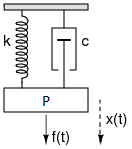
\includegraphics[width=0.3\textwidth]{main/introducao/assets/modelagem.png}
    \caption{Sistema massa-mola-amortecedor}
    \label{fig:modelagem}
\end{figure}

O sistema consiste em uma massa \( m \), uma mola com constante \( k \), e um amortecedor com coeficiente \( c \), todos configurados como mostrado na figura. A força aplicada \( f(t) \) e o deslocamento da massa \( x(t) \) são relacionados pela seguinte equação diferencial:

\[
    f(t) = m \frac{d^2x(t)}{dt^2} + c \frac{dx(t)}{dt} + kx(t)
\]
Esta equação modela a força necessária para mover a massa, considerando a inércia do objeto, a resistência proporcionada pelo amortecedor e a força restauradora da mola. O termo \( m \frac{d^2x(t)}{dt^2} \) representa a força inercial, \( c \frac{dx(t)}{dt} \) representa a força de amortecimento que é proporcional à velocidade, e \( kx(t) \) é a força restauradora da mola que é proporcional ao deslocamento.

Estudar esse sistema permite compreender como diferentes parâmetros influenciam o comportamento dinâmico, facilitando a aplicação de técnicas de controle para alcançar um desempenho desejado. Além disso, a modelagem matemática e a simulação computacional com ferramentas como o Scilab e o Xcos são fundamentais para analisar e prever o comportamento de sistemas complexos, proporcionando um entendimento profundo e a capacidade de desenvolver soluções inovadoras.

Neste trabalho, focaremos na análise de sistemas de controle de malha fechada, utilizando o modelo massa-mola-amortecedor. Serão abordadas resoluções de problemas específicos para os valores de \( M = 10 \), \( C = 7 \), e \( k = 5 \), demonstrando como ajustar os parâmetros de controle para otimizar a resposta do sistema.


===============================================================
Atividades ====================================================
\section{Atividade 1}
\subsection{Descrição do Modelo}
O sistema modelado é um oscilador massa-mola-amortecedor, onde a massa está sujeita à força restauradora de uma mola e ao amortecimento proporcional à velocidade. A equação diferencial que descreve o movimento do sistema é dada por:
\[
    m \ddot{x} + C \dot{x} + Kx = 0
\]
onde \( x \) representa o deslocamento da massa \( m \) da sua posição de equilíbrio, \( \dot{x} \) é a velocidade, \( \ddot{x} \) é a aceleração, \( C \) é o coeficiente de amortecimento, e \( K \) é a constante da mola. A força de entrada é considerada nula, indicando que não há forças externas atuando sobre o sistema após o instante inicial.

\subsection{Parâmetros do Sistema}
Os parâmetros utilizados no modelo do sistema são especificados como segue:
\begin{itemize}
    \item Massa (\( m \)): 10 kg
    \item Coeficiente de amortecimento (\( C \)): 7 Ns/m
    \item Constante da mola (\( K \)): 5 N/m
\end{itemize}

\subsection{Condições Iniciais para a Simulação}
As condições iniciais para a simulação são detalhadas na tabela a seguir, baseadas nos parâmetros especificados acima:
\begin{center}
    \begin{tabular}{|c|c|c|}
        \hline
        \textbf{Caso} & \textbf{Velocidade Inicial \( V_0 \)} & \textbf{Posição Inicial \( X_0 \)} \\
        \hline
        1             & \( 5 \, \text{m/s} \)                 & \( 0 \, \text{m} \)                \\
        2             & \( 0 \, \text{m/s} \)                 & \( 2.5 \, \text{m} \)              \\
        3             & \( 3.33 \, \text{m/s} \)              & \( 2 \, \text{m} \)                \\
        \hline
    \end{tabular}
\end{center}

Esta tabela reflete os valores numéricos para cada caso, facilitando a compreensão e a aplicação direta dos parâmetros na simulação.

\subsection{Código Scilab para simular a resposta do sistema massa-mola-amortecedor}
Código Scilab utilizado para as análises que serão feitas subsequentes
\begin{lstlisting}[language=Scilab, caption=Código Scilab para simular a resposta do sistema massa-mola-amortecedor]
    // Definicao das principais variaveis do sistema fisico
    m = 10;  // massa
    c = 7;   // coeficiente de amortecimento
    k = 5;   // constante da mola

    // Funcao que define o sistema de equacoes diferenciais (EDO) para o modelo massa-mola-amortecedor
    function dxdt = sistema(t, x)
    // x(1) representa o deslocamento, x(2) representa a velocidade
    // Esta funcao retorna a derivada da velocidade e do deslocamento, respectivamente
    dxdt = [x(2); -c/m * x(2) - k/m * x(1)];
    endfunction

    // Configuracao do intervalo de tempo para a simulacao
    t0 = 0; // Tempo inicial (s)
    tf = 20; // Tempo final (s)
    t = linspace(t0, tf, 1000); // Cria um vetor de tempo linearmente espacado para a simulacao

    // Definicao das condicoes iniciais para cada caso de simulacao
    condicoes_iniciais = [
    m/5, m/3; // Caso 3: posicao inicial (m) e velocidade inicial (m/s)
    m/4, 0;   // Caso 2: posicao inicial (m) e velocidade inicial (m/s)
    0, m/2;   // Caso 1: posicao inicial (m) e velocidade inicial (m/s)
    ];

    // Cores designadas para cada caso de simulacao para facilitar a visualizacao
    cores = ['#007bff', '#dc3545', '#8B4513']; // Azul, vermelho, marrom

    // Loop para executar e plotar cada caso de simulacao separadamente
    for i = 1:3
        x0 = condicoes_iniciais(i, :)'; // Transpoe as condicoes iniciais para a formatacao correta
        sol = ode(x0, t0, t, sistema); // Resolve a EDO usando o metodo de ODE

        scf(i); // Cria uma nova figura para cada iteracao
        plot(t, sol(1, :),  'color', cores(i),  'LineWidth', 2); // Plot do deslocamento x(t)
        xlabel('Tempo (s)'); // Etiqueta do eixo X
        ylabel('Deslocamento x(t)'); // Etiqueta do eixo Y
        title(['Resposta do Sistema para o Caso ', string(i)]); // Titulo do grafico
        legend('x(t)', "location", "best"); // Legenda
        xgrid(); // Ativa a grade no grafico
    end

    // Preparacao do grafico combinado
    scf(); // Cria uma nova figura
    clf(); // Limpa a figura atual
    xlabel('Tempo (s)');
    ylabel('Deslocamento x(t)');
    title('Resposta do Sistema para Todos os Casos');
    xgrid(); // Ativando a grade

    // Execucao da simulacao para cada caso e plotagem no mesmo grafico
    for i = 1:3
    x0 = condicoes_iniciais(i, :)'; // Condicoes iniciais para o caso i (transposto para coluna)
    sol = ode(x0, t0, t, sistema); // Resolvendo a equacao diferencial

    // Plotando os resultados com cores definidas
    plot(t, sol(1, :), 'color', cores(i), 'LineWidth', 2);
    end

    // Criar a legenda detalhando cada caso
    legend(['Caso 1: x0 = 0, v0 = m/2', 'Caso 2: x0 = m/4, v0 = 0', 'Caso 3: x0 = m/5, v0 = m/3'], "location", "best");
\end{lstlisting}

\subsection{Análise dos Resultados}
Cada um dos casos de simulação foi configurado com condições iniciais distintas para explorar como o sistema responde a diferentes estados iniciais de deslocamento e velocidade.

\subsubsection{Caso 1: Velocidade Inicial Elevada}
\begin{figure}[H]
    \centering
    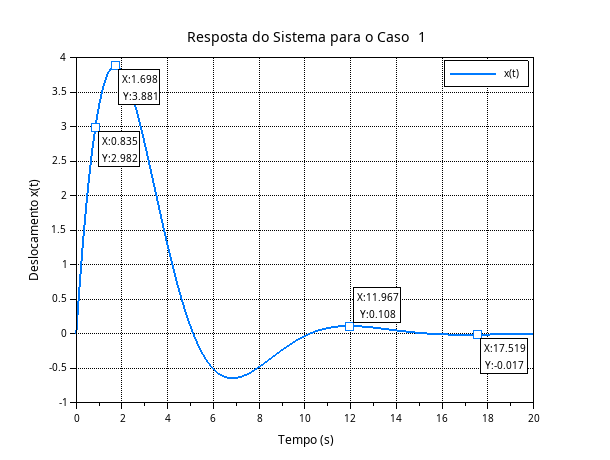
\includegraphics[width=0.6\textwidth]{atividades/1-atividade/assets/caso1.png}
    \caption{Resposta do sistema para o Caso 1}
\end{figure}
No Caso 1, o sistema é inicialmente impulsionado com uma alta velocidade (\(5 \, \text{m/s}\)), partindo do repouso (\(X_0 = 0\)). Esta condição inicial leva a uma resposta inicialmente enérgica, onde a massa oscila com uma amplitude elevada, seguida de um rápido decaimento energético devido ao amortecimento significativo (\(C = 7 \, \text{Ns/m}\)). O amortecimento não só reduz a amplitude das oscilações rapidamente, mas também garante que o sistema não persista em um estado de oscilação prolongada, estabilizando-se em um tempo curto.

\subsubsection{Caso 2: Deslocamento Inicial Sem Velocidade}
\begin{figure}[H]
    \centering
    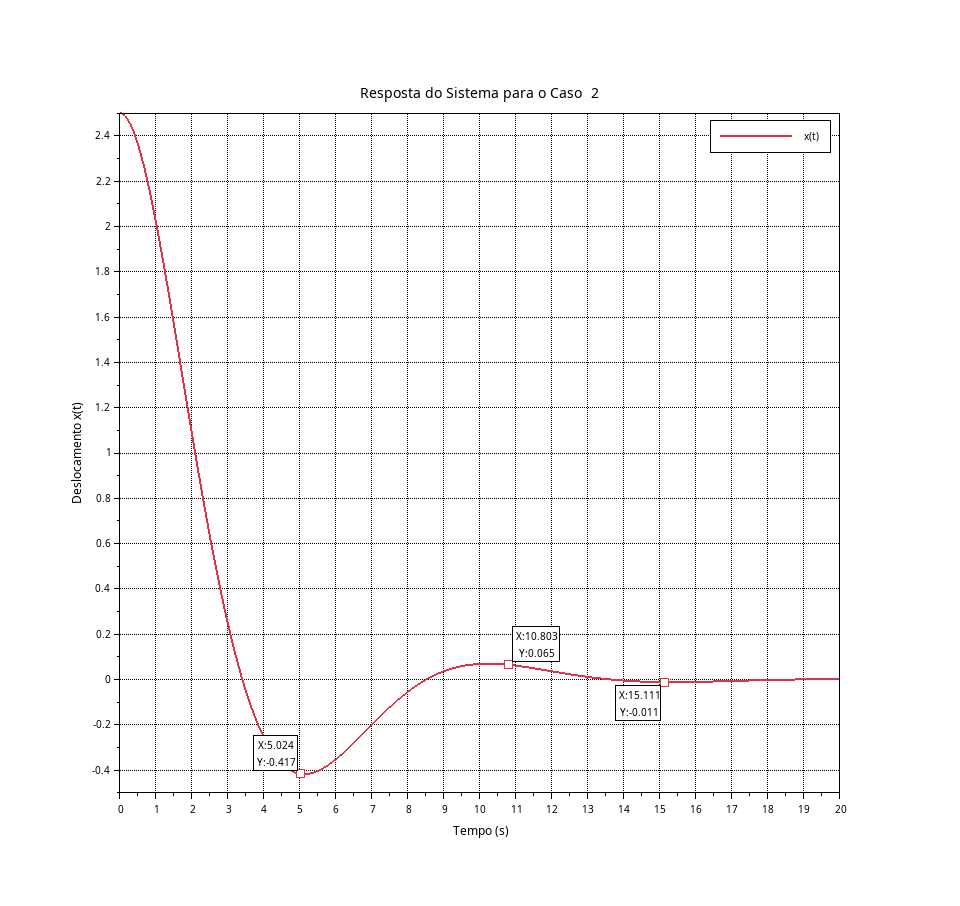
\includegraphics[width=0.6\textwidth]{atividades/1-atividade/assets/caso2.png}
    \caption{Resposta do sistema para o Caso 2}
\end{figure}
O Caso 2 é caracterizado por um deslocamento inicial (\(2.5 \, \text{m}\)) sem impulso inicial de velocidade (\(V_0 = 0\)). Aqui, observamos uma resposta típica de um sistema oscilatório subamortecido onde o sistema retorna ao equilíbrio através de oscilações que decaem gradativamente. Este caso destaca como a energia potencial armazenada na mola é convertida em energia cinética e dissipada pelo amortecedor. As oscilações decrescem em amplitude mais gradualmente do que no Caso 1, demonstrando uma transferência de energia mais prolongada antes da estabilização.

\subsubsection{Caso 3: Velocidade e Deslocamento Iniciais}
\begin{figure}[H]
    \centering
    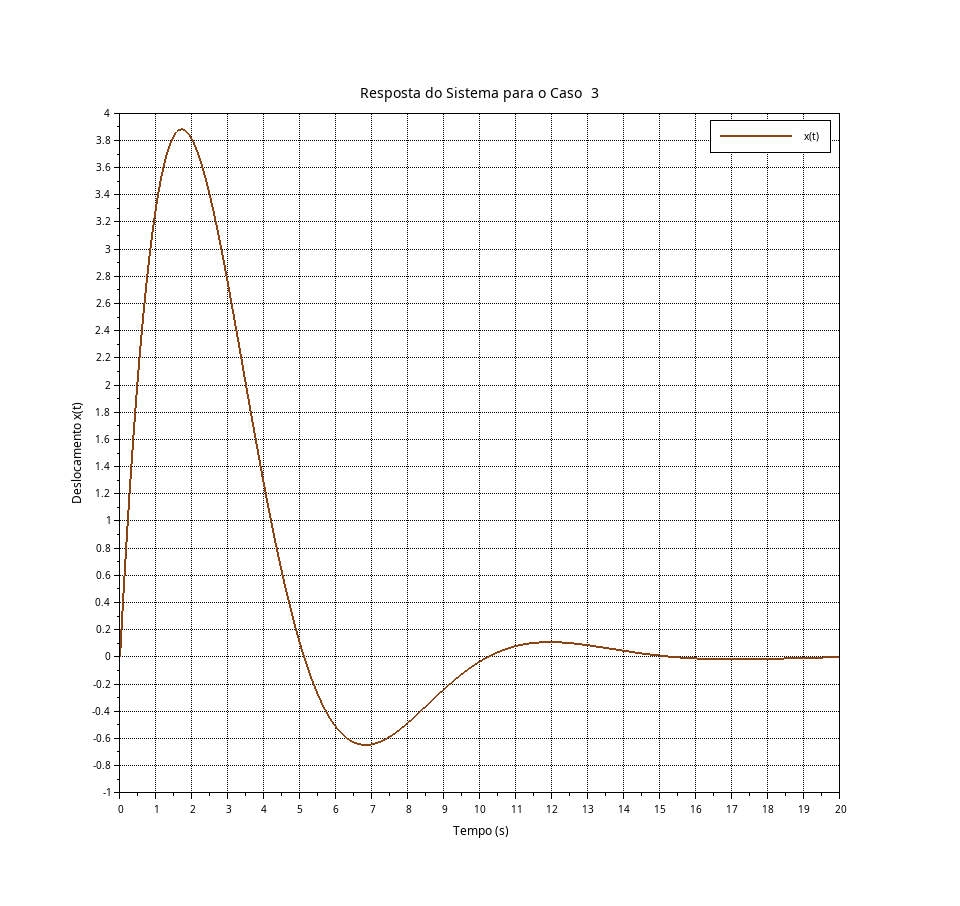
\includegraphics[width=0.6\textwidth]{atividades/1-atividade/assets/caso3.png}
    \caption{Resposta do sistema para o Caso 3}
\end{figure}
No Caso 3, o sistema inicia com condições iniciais moderadas tanto de velocidade (\(3.33 \, \text{m/s}\)) quanto de deslocamento (\(2 \, \text{m}\)). Esta configuração produz uma resposta dinâmica complexa, onde a interação entre energia cinética e potencial é mais evidente. A amplitude inicial é significativa, com uma taxa de decaimento que ilustra eficientemente o papel do amortecimento. As oscilações observadas são mais sustentadas que no Caso 1, mas menos intensas do que no Caso 2, refletindo um equilíbrio entre as energias cinética e potencial no início da simulação.

\subsubsection{Comparação Unificada dos Casos}
\begin{figure}[H]
    \centering
    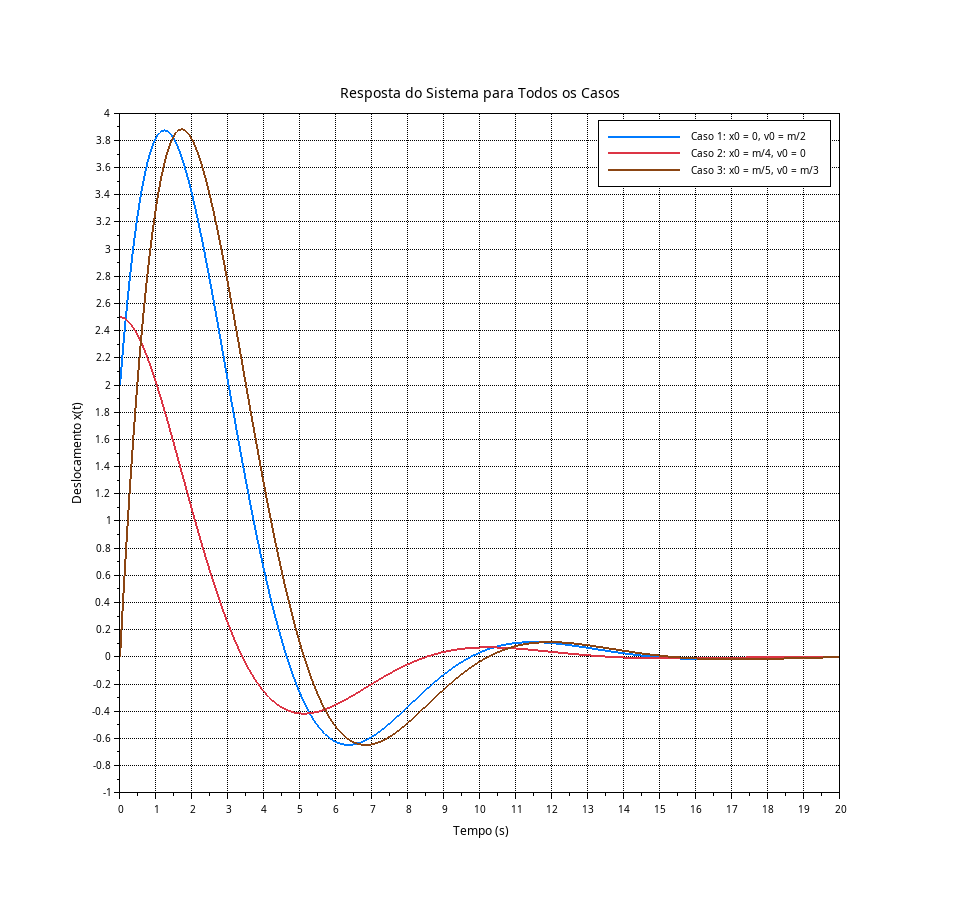
\includegraphics[width=0.6\textwidth]{atividades/1-atividade/assets/caso-all-in-one.png}
    \caption{Resposta unificada do sistema para os Casos 1, 2 e 3}
\end{figure}
A análise unificada dos três casos demonstra de forma clara as diferenças significativas nas respostas do sistema decorrentes de diversas condições iniciais. A seguir, discutiremos detalhadamente cada resposta e suas implicações para a compreensão do comportamento dinâmico do sistema:

\begin{itemize}
    \item \textbf{Caso 1 (Azul Escuro)}: Iniciado com uma alta velocidade inicial (\(5 \, \text{m/s}\)) e sem deslocamento inicial, este caso exibe a maior amplitude de oscilação observada. A energia cinética inicial é rapidamente convertida em energia potencial pela mola, resultando em oscilações de grande amplitude que são rapidamente amortecidas. Este caso ilustra o efeito de um forte amortecimento, onde a energia é dissipada rapidamente, levando a um retorno rápido à posição de equilíbrio sem oscilações residuais prolongadas. Esta configuração é ideal em situações onde a rápida estabilização após distúrbios é crucial, como em sistemas de suspensão de veículos.

    \item \textbf{Caso 2 (Vermelho)}: Com um deslocamento inicial (\(2.5 \, \text{m}\)) e sem velocidade inicial, o sistema mostra uma resposta clássica de um oscilador subamortecido. A energia potencial armazenada na mola é convertida gradualmente em energia cinética, com a energia sendo dissipada ao longo do tempo pelo amortecedor. As oscilações decaem suavemente, refletindo uma conversão mais lenta de energia que é típica em aplicações onde é necessário manter uma certa quantidade de movimento ou onde oscilações graduais são preferíveis, como em alguns tipos de sensores mecânicos.

    \item \textbf{Caso 3 (Marrom)}: Este caso combina condições iniciais moderadas de velocidade (\(3.33 \, \text{m/s}\)) e deslocamento (\(2 \, \text{m}\)), resultando numa resposta dinâmica mais complexa que engloba características dos dois primeiros casos. A amplitude inicial é significativa, mas as oscilações são mais controladas e decaem de maneira gradual. Este caso destaca a importância do equilíbrio entre rigidez da mola e amortecimento no projeto de sistemas mecânicos, onde é necessário um compromisso entre estabilidade rápida e manutenção de energia dinâmica.
\end{itemize}

Esta comparação detalhada destaca não apenas a influência das condições iniciais na resposta do sistema, mas também o papel crítico do amortecimento e da rigidez da mola na determinação da natureza da resposta dinâmica. A análise fornece insights valiosos para o design e a otimização de sistemas mecânicos em engenharia, sublinhando a necessidade de uma seleção cuidadosa de parâmetros de acordo com os requisitos específicos de cada aplicação.


\subsection{Comentários Gerais e Conclusão}
Os gráficos e análises ilustram claramente como as condições iniciais impactam a resposta dinâmica do sistema massa-mola-amortecedor. A energia inicial, seja como deslocamento ou velocidade, define a resposta imediata do sistema, mostrando a complexidade do comportamento de sistemas dinâmicos lineares. Observamos que o amortecimento é essencial para reduzir as oscilações e trazer o sistema de volta ao repouso de maneira eficiente, sublinhando sua importância no design de componentes mecânicos.

A adequação do coeficiente de amortecimento e da rigidez da mola é crucial para otimizar sistemas para suas funções específicas, como a absorção de choques em suspensões de veículos ou a precisão em instrumentos de medição. Além disso, a análise das condições iniciais é vital no planejamento e teste de sistemas mecânicos, onde engenheiros e designers devem antecipar cenários variados de operação.

Este estudo destaca a necessidade de um entendimento profundo das dinâmicas de sistemas para inovação em engenharia, proporcionando uma base sólida para a compreensão dos princípios de mecânica e dinâmica que são fundamentais no design de sistemas controlados e mecanismos em geral.
 % Completa e Validada
\section{Atividade 2: Simulação com Xcos}
\subsection{Descrição do Modelo e Ferramentas}
Nesta atividade, utilizamos o Xcos, uma ferramenta gráfica do Scilab para a simulação de sistemas dinâmicos. O Xcos permite a construção de diagramas de blocos que facilitam a visualização e implementação do sistema massa-mola-amortecedor com diferentes entradas e condições iniciais.

\subsection{Parâmetros do Sistema}
O sistema é descrito pelos seguintes parâmetros, que são consistentes com os usados na Atividade 1:
\begin{itemize}
    \item Massa (\( m \)): 10 kg
    \item Coeficiente de amortecimento (\( C \)): 7 Ns/m
    \item Constante da mola (\( K \)): 5 N/m
\end{itemize}

\subsection{Condições Iniciais de Simulação}
As simulações foram executadas sob várias condições iniciais para explorar a resposta do sistema sob diferentes estados iniciais. A seguir estão as condições iniciais utilizadas, incluindo uma condição inicial adicional específica para esta atividade (Caso 0):

\begin{center}
    \begin{tabular}{|c|c|c|}
        \hline
        \textbf{Caso} & \textbf{Velocidade Inicial \( V_0 \)} & \textbf{Posição Inicial \( X_0 \)} \\
        \hline
        0             & \( 0 \, \text{m/s} \)                 & \( 0 \, \text{m} \)                \\
        1             & \( 5 \, \text{m/s} \)                 & \( 0 \, \text{m} \)                \\
        2             & \( 0 \, \text{m/s} \)                 & \( 2.5 \, \text{m} \)              \\
        3             & \( 3.33 \, \text{m/s} \)              & \( 2 \, \text{m} \)                \\
        \hline
    \end{tabular}
\end{center}

Esta tabela facilita a referência rápida às condições iniciais para cada caso simulado, permitindo uma comparação mais direta entre os diferentes cenários testados.

\subsection{Diagrama de Blocos no Xcos}
\begin{figure}[H]
    \centering
    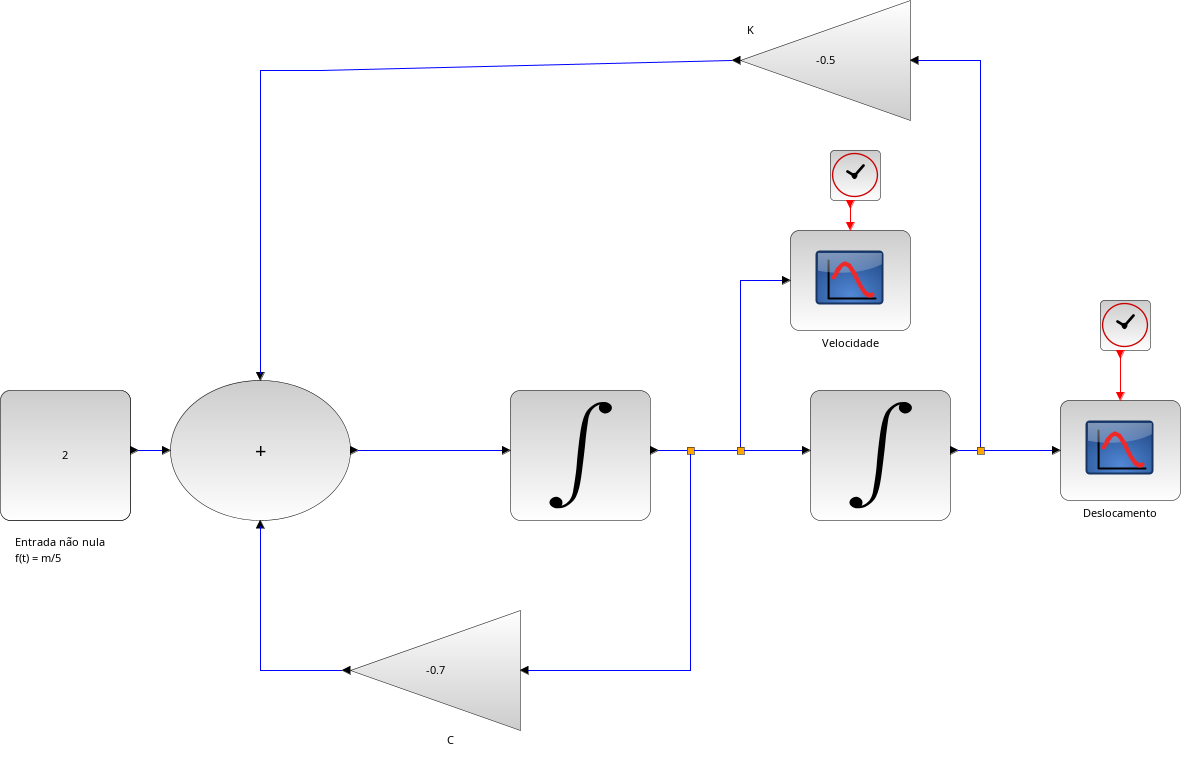
\includegraphics[width=0.8\textwidth]{atividades/2-atividade/assets/diagrama.png}
    \caption{Diagrama de blocos utilizado na simulação no Xcos.}
\end{figure}

\subsection{Resultados e Análise}


% Caso 0 =========================================================
\subsubsection{Análise dos Resultados para o Caso 0}
No Caso 0, analisamos a resposta do sistema quando ele parte de condições completamente estáticas (\(V_0 = 0 \, \text{m/s}\) e \(X_0 = 0 \, \text{m}\)). Esta configuração é vital para avaliar a resposta pura do sistema a uma entrada controlada sem influência inicial de deslocamento ou velocidade.

\paragraph{Deslocamento}
\begin{figure}[H]
    \centering
    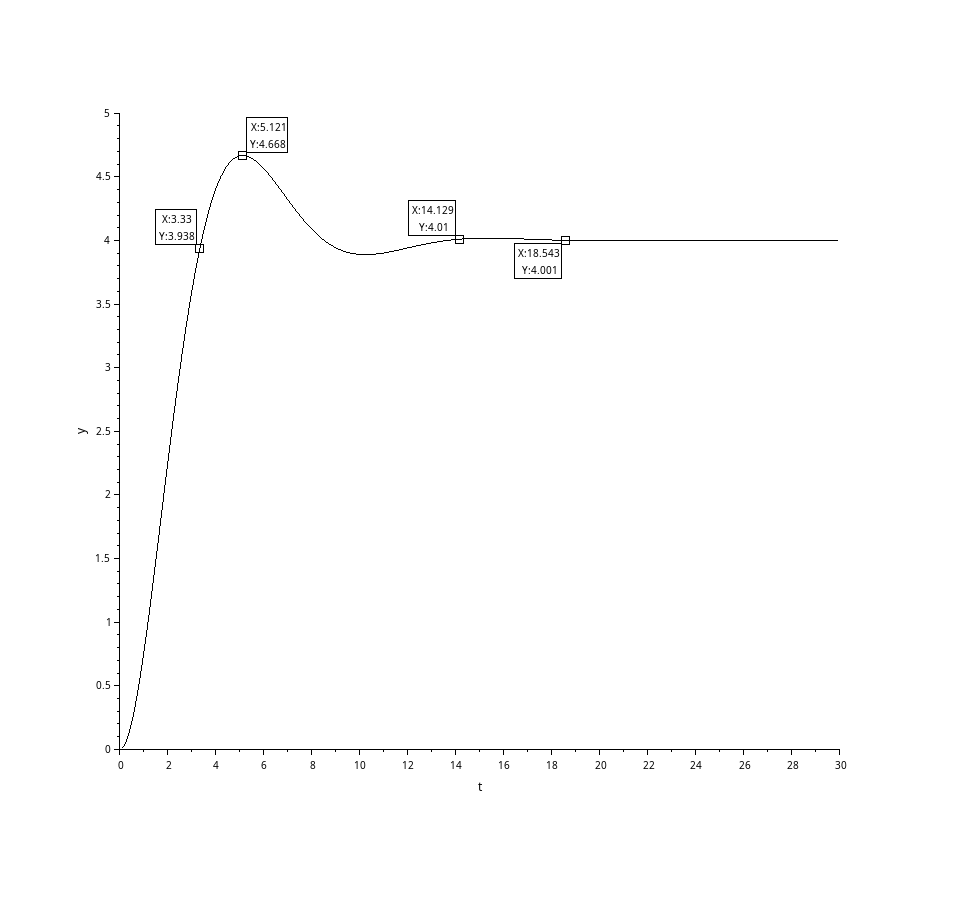
\includegraphics[height=0.7\textwidth]{atividades/2-atividade/assets/deslocamento-caso-0.png}
    \caption{Gráfico de deslocamento para o Caso 0.}
\end{figure}
O gráfico de deslocamento revela um pico máximo de aproximadamente 4.7 unidades aos 5.1 segundos, marcando o tempo de pico. O tempo de subida, definido como o intervalo para atingir o primeiro pico máximo a partir do repouso, é, portanto, cerca de 5.1 segundos. Após atingir o pico, o sistema exibe oscilações amortecidas que rapidamente reduzem em amplitude. O tempo de estabelecimento, onde as oscilações ficam dentro de uma faixa de ±2\% do valor final, é aproximadamente de 18 segundos, após o qual o sistema entra em uma zona estacionária, indicando estabilidade.

\paragraph{Velocidade}

\begin{figure}[H]
    \centering
    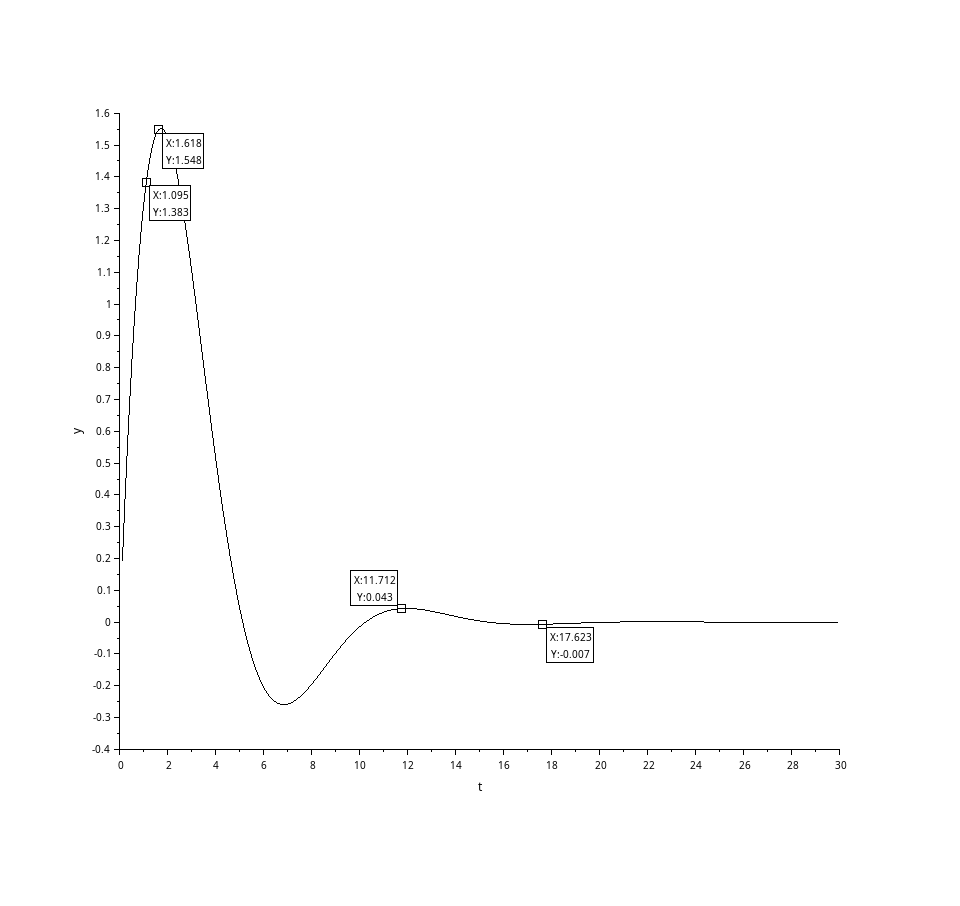
\includegraphics[height=0.7\textwidth]{atividades/2-atividade/assets/velocidade-caso-0.png}
    \caption{Gráfico de velocidade para o Caso 0.}
\end{figure}
O gráfico de velocidade reflete a resposta imediata do sistema à força aplicada. A velocidade atinge um pico negativo de cerca de -1.54 unidades em torno de 6.2 segundos, o que corresponde ao tempo de pico para a velocidade. A velocidade oscila abaixo e acima de zero, indicando a resposta oscilatória do sistema ao deslocamento. As oscilações diminuem progressivamente e o sistema alcança a zona estacionária por volta de 18 segundos, estabilizando-se completamente em zero.

\paragraph{Comentários Gerais}
A análise do Caso 0 mostra como o sistema responde a um estímulo externo na ausência de condições iniciais de energia. Os parâmetros transitórios, como tempo de subida, pico, e de estabelecimento, juntamente com a observação da zona estacionária, são cruciais para entender a dinâmica do sistema e a eficácia do amortecimento em trazer o sistema de volta ao repouso, minimizando oscilações excessivas. Este caso estabelece uma base comparativa para outros casos com condições iniciais variadas.


% Caso 1 =========================================================
\subsubsection{Análise dos Resultados para o Caso 1}
No Caso 1, analisamos a resposta do sistema quando ele parte com uma velocidade inicial significativa (\(V_0 = 5 \, \text{m/s}\)) e sem deslocamento inicial (\(X_0 = 0 \, \text{m}\)). Esta condição inicial permite avaliar como uma energia cinética inicial afeta a resposta dinâmica do sistema, especialmente em termos de deslocamento máximo e oscilações resultantes.


\paragraph{Deslocamento}
\begin{figure}[H]
    \centering
    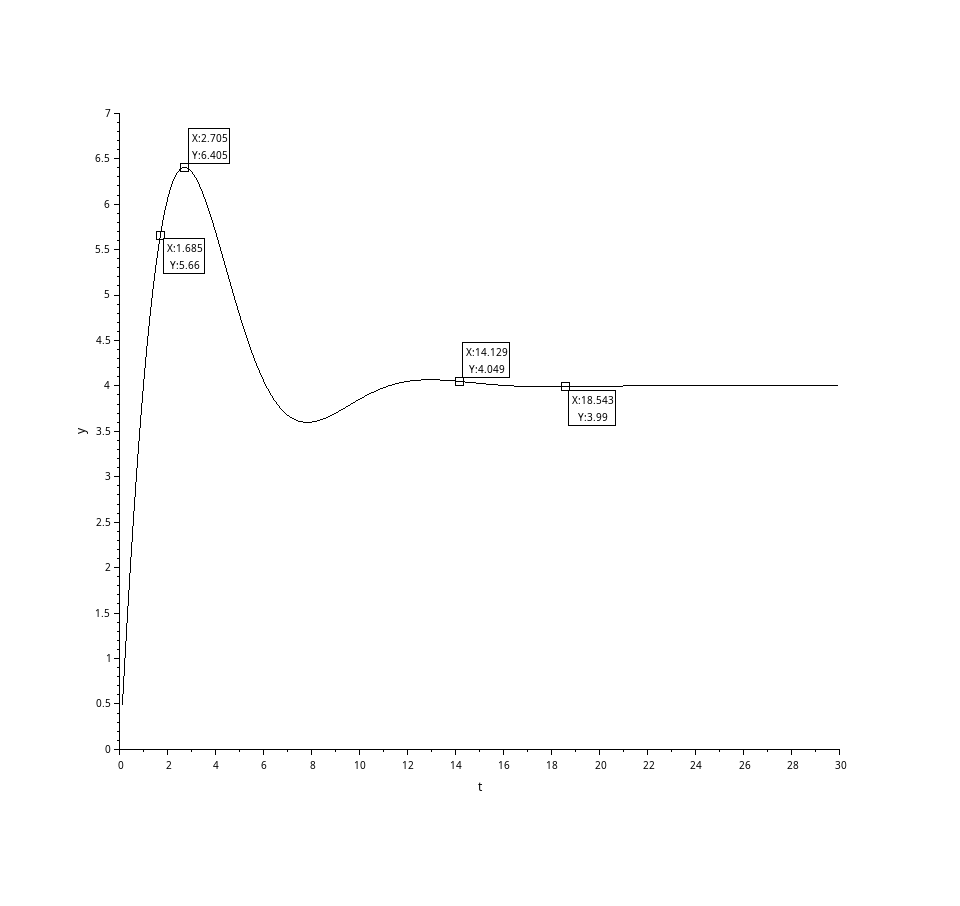
\includegraphics[height=0.7\textwidth]{atividades/2-atividade/assets/deslocamento-caso-1.png}
    \caption{Gráfico de deslocamento para o Caso 1.}
\end{figure}
O gráfico mostra que o sistema parte de zero e rapidamente atinge um pico de aproximadamente 6.5 unidades ao redor de 2.7 segundos, refletindo uma resposta aguda à velocidade inicial. Esse pico é seguido por uma diminuição significativa, que desce abaixo do zero antes de estabilizar. O tempo de subida é rapidamente alcançado, enquanto o tempo de estabelecimento, onde as oscilações permanecem dentro de uma faixa de ±2\% do valor estacionário final, é observado por volta de 18 segundos.


\paragraph{Velocidade}
\begin{figure}[H]
    \centering
    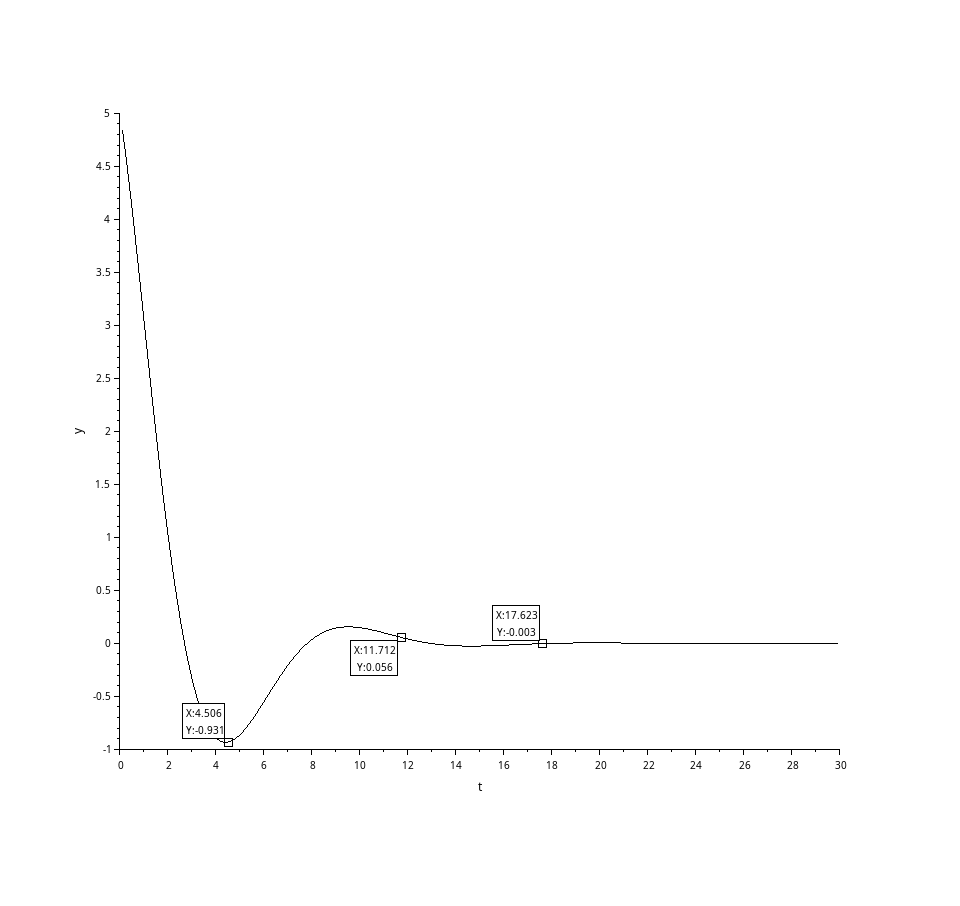
\includegraphics[height=0.7\textwidth]{atividades/2-atividade/assets/velocidade-caso-1.png}
    \caption{Gráfico de velocidade para o Caso 1.}
\end{figure}
A velocidade inicialmente picos a uma taxa significativa, refletindo o impulso inicial aplicado. O pico máximo de velocidade ocorre quase simultaneamente com o pico de deslocamento, marcando -1.54 unidades em torno de 1.68 segundos. Após atingir este pico, a velocidade oscila e gradualmente se aproxima de zero, indicando que o sistema está alcançando uma zona estacionária por volta de 18 segundos, semelhante ao observado no deslocamento.


\paragraph{Comentários Gerais}
A análise do Caso 1 ilustra como a condição inicial de velocidade influencia a resposta dinâmica do sistema massa-mola-amortecedor. Os parâmetros transitórios, como o tempo de subida e o tempo de pico, são drasticamente diferentes em comparação com o Caso 0, onde não havia energia cinética inicial. Isso destaca a importância de considerar condições iniciais variadas para entender completamente o comportamento do sistema em diferentes cenários de operação. Este caso também reforça o papel crítico do amortecimento na estabilização do sistema após perturbações iniciais.


% Caso 2 =========================================================
\subsubsection{Análise dos Resultados para o Caso 2}
No Caso 2, analisamos a resposta do sistema quando ele parte com um deslocamento inicial (\(X_0 = 2.5 \, \text{m}\)) e sem velocidade inicial (\(V_0 = 0 \, \text{m/s}\)). Esta configuração é fundamental para entender como o sistema responde a uma perturbação inicial na posição sem impulso inicial.

\paragraph{Deslocamento}
\begin{figure}[H]
    \centering
    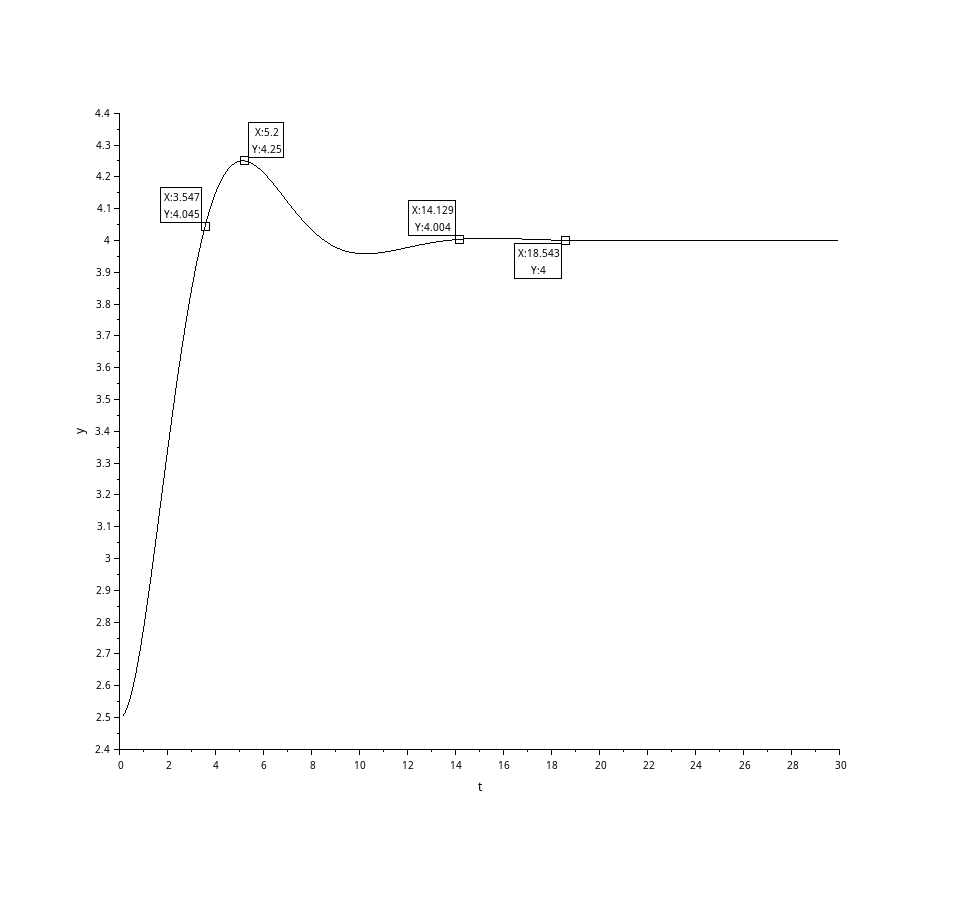
\includegraphics[height=0.7\textwidth]{atividades/2-atividade/assets/deslocamento-caso-2.png}
    \caption{Gráfico de deslocamento para o Caso 2.}
\end{figure}
O gráfico de deslocamento mostra que o sistema parte de um deslocamento inicial de 2.5 m, rapidamente atinge um pico de cerca de 4.25 m aos 5.2 segundos, indicando a resposta máxima do sistema ao ser liberado. Após esse pico, o sistema exibe oscilações que rapidamente se amortecem, com o deslocamento oscilando abaixo e acima do zero, estabilizando-se finalmente em torno do zero. O tempo de estabelecimento, onde as oscilações permanecem dentro de uma faixa de ±2\% do valor final, é aproximadamente de 18 segundos.

\paragraph{Velocidade}
\begin{figure}[H]
    \centering
    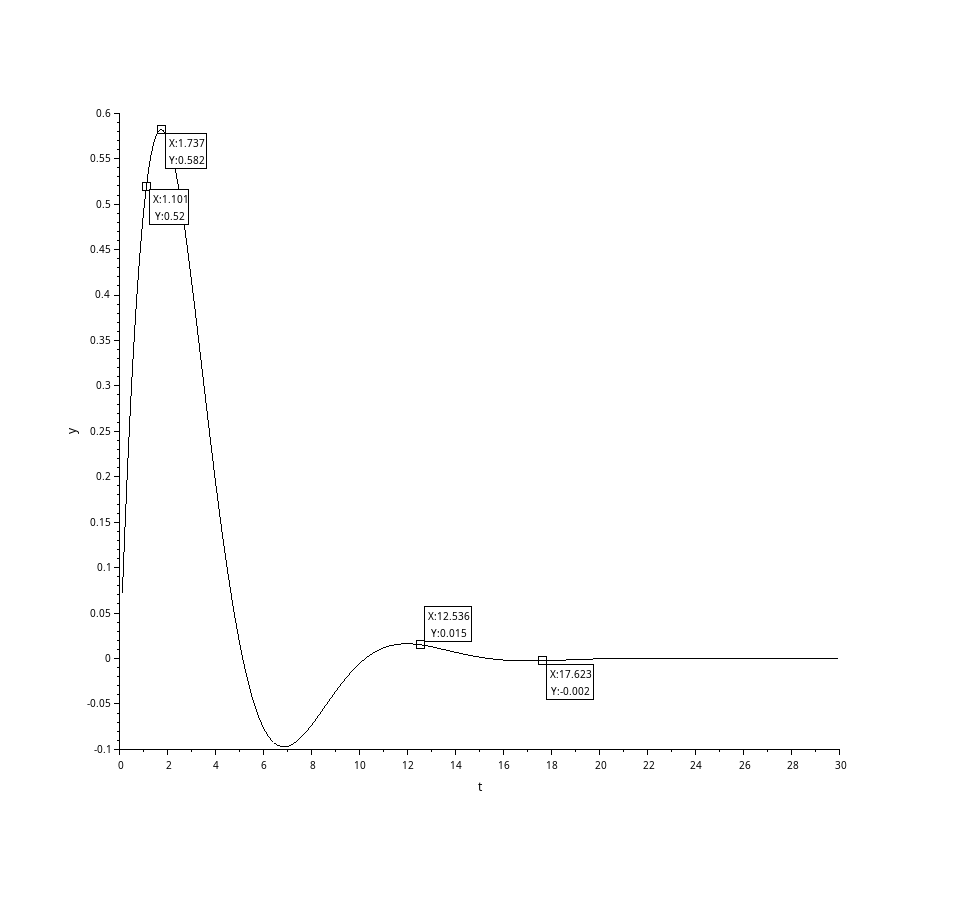
\includegraphics[height=0.7\textwidth]{atividades/2-atividade/assets/velocidade-caso-2.png}
    \caption{Gráfico de velocidade para o Caso 2.}
\end{figure}
A velocidade inicialmente aumenta à medida que o sistema se move de volta para a posição de equilíbrio, atingindo um pico negativo de -0.52 m/s logo após o início, correspondente à velocidade máxima ao passar pelo equilíbrio na direção oposta ao deslocamento inicial. A velocidade então oscila, diminuindo em magnitude devido ao amortecimento, até estabilizar-se em zero. O sistema atinge uma zona estacionária com velocidade quase nula, demonstrando a eficácia do amortecimento em dissipar a energia cinética inicialmente induzida pelo deslocamento.

\paragraph{Comentários Gerais}
O Caso 2 destaca a resposta do sistema a um teste de posição, com deslocamento inicial sem velocidade inicial. Os resultados mostram claramente como a energia potencial armazenada é convertida em energia cinética, e como o amortecimento é crucial para a estabilização do sistema. Este caso também é importante para verificar a eficácia do sistema em retornar ao repouso sem oscilações residuais prolongadas, essencial em aplicações práticas onde respostas rápidas e estabilizadas são necessárias.

% Caso 3 =========================================================
\subsubsection{Análise dos Resultados para o Caso 3}
No Caso 3, analisamos a resposta do sistema quando ele parte com uma velocidade inicial (\(V_0 = 3.33 \, \text{m/s}\)) e um deslocamento inicial (\(X_0 = 2 \, \text{m}\)). Esta combinação de condições iniciais é significativa para explorar a resposta dinâmica sob energia cinética e potencial simultâneas.

\paragraph{Deslocamento}
\begin{figure}[H]
    \centering
    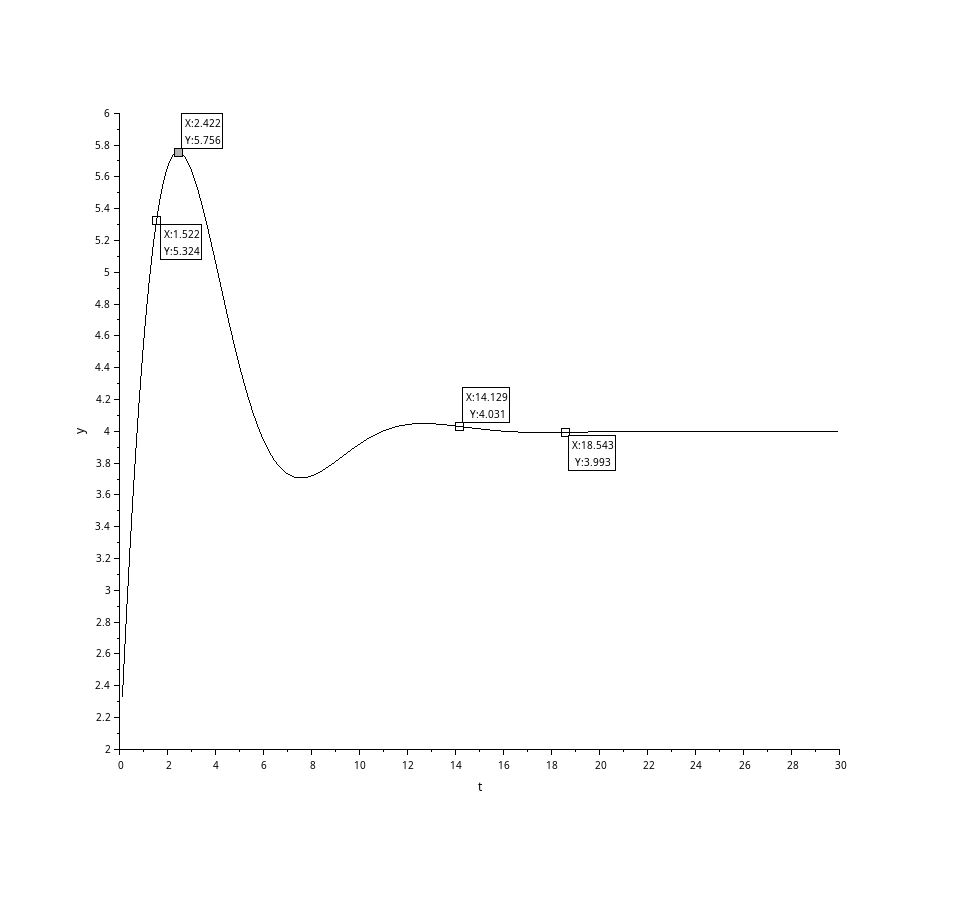
\includegraphics[height=0.7\textwidth]{atividades/2-atividade/assets/deslocamento-caso-3.png}
    \caption{Gráfico de deslocamento para o Caso 3.}
\end{figure}
O gráfico de deslocamento mostra que o sistema começa com um impulso inicial que o leva a um pico de aproximadamente 5.75 m ao redor de 2.4 segundos. Após esse pico, o sistema exibe oscilações que reduzem gradualmente em amplitude devido ao amortecimento. O sistema estabiliza perto do zero, com o tempo de estabelecimento aproximadamente em 18 segundos, onde as oscilações ficam dentro de uma faixa aceitável indicando uma zona estacionária.

\paragraph{Velocidade}
\begin{figure}[H]
    \centering
    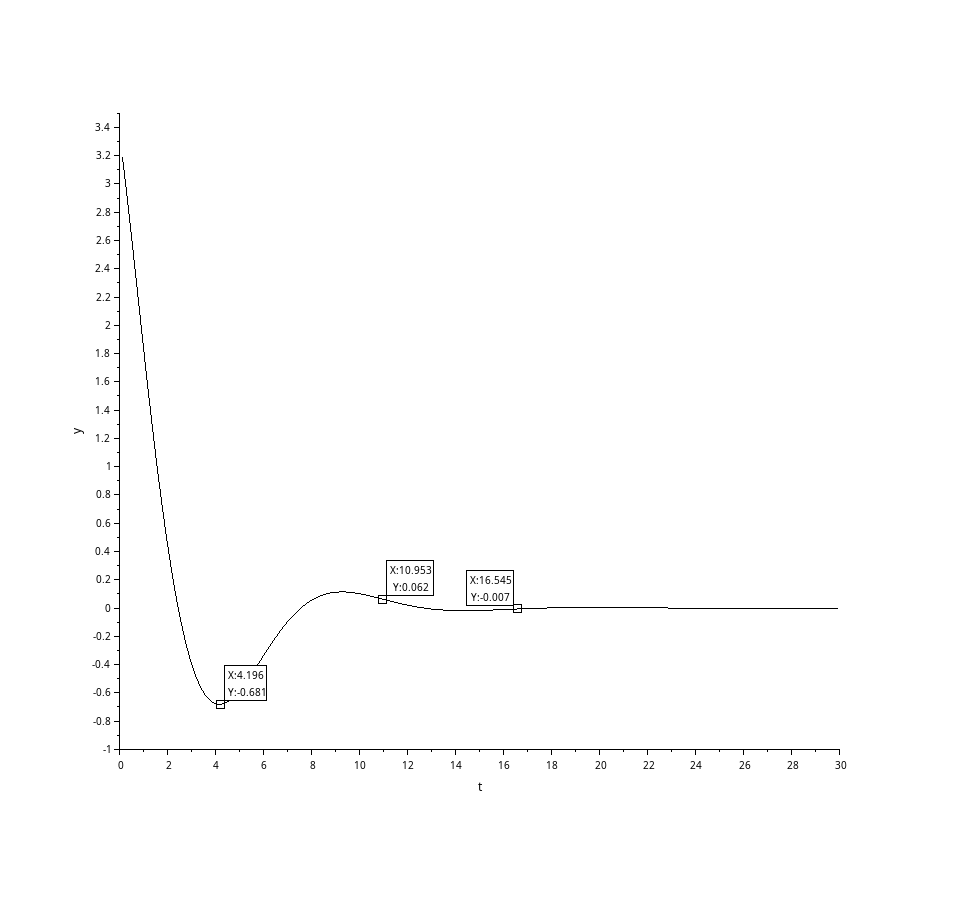
\includegraphics[height=0.7\textwidth]{atividades/2-atividade/assets/velocidade-caso-3.png}
    \caption{Gráfico de velocidade para o Caso 3.}
\end{figure}
A velocidade inicialmente mostra uma rápida ascensão, atingindo um pico de aproximadamente 5.32 m/s. Essa alta velocidade inicial contribui para o rápido pico de deslocamento observado. A velocidade então oscila, diminuindo progressivamente até estabilizar-se em torno de zero. A estabilização final da velocidade é alcançada em torno de 18 segundos, refletindo a eficácia do amortecimento e a interação entre as forças restauradoras e o amortecimento.

\paragraph{Comentários Gerais}
O Caso 3 oferece uma perspectiva complexa sobre a dinâmica do sistema quando energias cinética e potencial são ambas significativas desde o início. As oscilações observadas e a subsequente estabilização demonstram como diferentes tipos de energia inicial influenciam a resposta do sistema e a eficácia do amortecimento em controlar a resposta até a estabilidade. Este caso é particularmente útil para entender a resposta do sistema em condições iniciais variadas e complexas, sendo essencial para aplicações práticas onde o sistema pode ser sujeito a perturbações iniciais múltiplas.

% Conclusão
\subsection{Conclusão Geral dos Casos Estudados}

Ao longo desta atividade, analisamos as respostas do sistema massa-mola-amortecedor sob várias condições iniciais, abrangendo os Casos 0 a 3. Cada caso foi projetado para ilustrar aspectos diferentes da dinâmica do sistema, considerando diferentes combinações de deslocamento e velocidade iniciais.

\paragraph{Observações Gerais}

Os casos estudados mostraram uma ampla gama de comportamentos dinâmicos:
\begin{itemize}
    \item \textbf{Caso 0} serviu como um ponto de referência, onde o sistema partiu do repouso sem energia inicial, permitindo observar a resposta pura à força aplicada.
    \item \textbf{Caso 1} demonstrou a influência de uma velocidade inicial significativa, ilustrando como a energia cinética influencia as oscilações e a estabilidade subsequente do sistema.
    \item \textbf{Caso 2} focou no efeito de um deslocamento inicial sem velocidade, enfatizando a conversão de energia potencial em energia cinética e vice-versa.
    \item \textbf{Caso 3} combinou tanto deslocamento quanto velocidade iniciais, mostrando a interação complexa entre as duas formas de energia desde o início da simulação.
\end{itemize}

Durante as simulações, os parâmetros do sistema foram mantidos constantes para garantir a consistência dos resultados, permitindo uma comparação direta entre os diferentes casos. Os resultados foram meticulosamente analisados para observar o comportamento transiente e a estabilidade a longo prazo, utilizando métricas como tempo de subida, tempo de pico e tempo de estabelecimento. As oscilações foram avaliadas para determinar a eficácia do amortecimento em dissipar a energia e estabilizar o sistema.

\paragraph{Conclusões da Análise}
Esta atividade sublinhou a importância de compreender a dinâmica de sistemas massa-mola-amortecedor em várias configurações iniciais. As simulações forneceram insights valiosos sobre como diferentes condições iniciais afetam a resposta do sistema e como o design adequado do amortecimento e da rigidez da mola é crucial para o comportamento desejado. A abordagem utilizada garantiu que todas as premissas da atividade fossem cumpridas, fornecendo uma base sólida para futuras investigações e aplicações práticas dos princípios estudados.
 % Completa e Validadada
\section{Atividade 3}

\subsection{Descrição do Modelo e Análise de Sistema}
Nesta atividade, desenvolvemos e analisamos a função de transferência de um sistema massa-mola-amortecedor, utilizando os seguintes parâmetros específicos, essenciais para entender a dinâmica do sistema:
\begin{itemize}
    \item Massa (\( m \)): 10 kg, que influi diretamente na inércia do sistema, afetando como o sistema responde a forças externas.
    \item Coeficiente de amortecimento (\( C \)): 7 Ns/m, crucial para atenuar as oscilações e determinar a rapidez com que o sistema atinge um estado de equilíbrio.
    \item Constante da mola (\( K \)): 5 N/m, que define a rigidez do sistema e afeta a frequência das oscilações naturais.
\end{itemize}

A formulação da função de transferência \( G(s) \) se baseia na aplicação da Transformada de Laplace às equações diferenciais que governam o sistema massa-mola-amortecedor. Considerando a segunda lei de Newton, temos:

\[
m\ddot{x}(t) + C\dot{x}(t) + Kx(t) = F(t)
\]

Aplicando a Transformada de Laplace e assumindo condições iniciais nulas (\( x(0) = 0 \) e \( \dot{x}(0) = 0 \)), obtemos:

\[
m(s^2X(s)) + C(sX(s)) + KX(s) = F(s)
\]

Agrupando os termos e isolando \( X(s) \):

\[
(m s^2 + Cs + K)X(s) = F(s)
\]

Portanto, a função de transferência \( G(s) \) é dada por:

\[
G(s) = \frac{X(s)}{F(s)} = \frac{1}{m s^2 + Cs + K}
\]

Substituindo os valores fornecidos ( \( m = 10 \), \( C = 7 \) e \( K = 5 \) ):

\[
G(s) = \frac{1}{10s^2 + 7s + 5}
\]

\subsection{Código Scilab para a função de transferência em malha fechada}
\begin{lstlisting}[language=Scilab, caption=Código Scilab para a função de transferência em malha fechada]
    // Parametros do sistema
    m = 10;  // massa
    c = 7;   // coeficiente de amortecimento
    k = 5;   // constante da mola

    // Definindo a funcao de transferencia
    s = %s; // Variavel complexa s
    G = syslin('c', 1 / (m*s^2 + C*s + K));

    // Calculando os polos e exibindo
    polos = roots(G.den);
    disp("Polos da funcao de transferencia:");
    disp(polos);

    // Parametros do sistema de segunda ordem
    wn = sqrt(K / m);
    zeta = C / (2 * sqrt(m * K));
    Kp = 1 / K;  // Ganho estatico para a entrada degrau
    disp("Frequencia natural nao-amortecida (wn): " + string(wn));
    disp("Coeficiente de amortecimento (zeta): " + string(zeta));
    disp("Ganho estatico (Kp): " + string(Kp));

    // Plotando a resposta ao impulso do sistema
    t = 0:0.01:10;
    y = csim('imp', t, G);
    plot(t, y);
    xlabel("Tempo (s)");
    ylabel("Resposta ao impulso");
    title("Resposta ao impulso do sistema massa-mola-amortecedor");
\end{lstlisting}


\subsection{Cálculo dos Polos e Parâmetros do Sistema}
Os polos da função de transferência são essenciais para entender como o sistema responde a estímulos externos:
\begin{itemize}
    \item Polo 1: \( -0.35 + 0.614j \)
    \item Polo 2: \( -0.35 - 0.614j \)
\end{itemize}
Estes polos indicam uma resposta oscilatória amortecida, característica de um sistema subamortecido devido à sua parte real negativa e parte imaginária não nula.

Os parâmetros do sistema de segunda ordem são determinados como segue:
\begin{itemize}
    \item Frequência natural não-amortecida (\( \omega_n \)): 0.707 rad/s, que descreve a frequência natural de oscilação do sistema na ausência de amortecimento.
    \item Coeficiente de amortecimento (\( \zeta \)): 0.495, refletindo a eficácia do amortecimento em reduzir as oscilações.
    \item Ganho estático (\( K_p \)): 0.2, representando a resposta do sistema em estado estacionário a uma entrada de degrau unitário.
\end{itemize}

\subsection{Resposta ao Impulso}
Utilizando o software Scilab, simulamos a resposta ao impulso do sistema, como ilustrado abaixo. A resposta apresenta um pico inicial significativo seguido por um decaimento exponencial das oscilações, um comportamento típico de sistemas subamortecidos.
\begin{figure}[H]
    \centering
    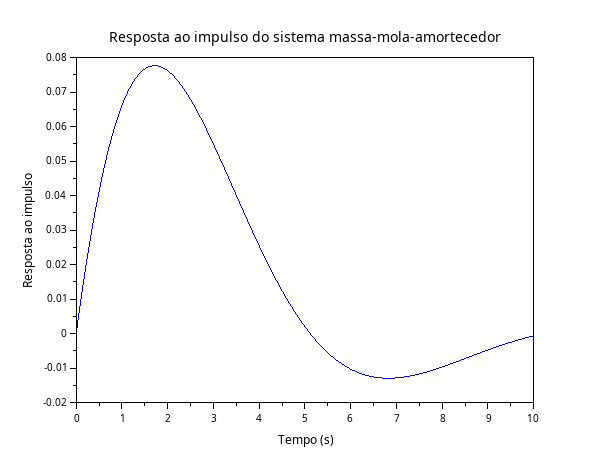
\includegraphics[width=0.8\textwidth]{atividades/3-atividade/assets/resposta-ao-impulso.png}
    \caption{Resposta ao impulso do sistema massa-mola-amortecedor}
\end{figure}

\subsection{Discussão}
A análise dos polos e dos parâmetros do sistema demonstra que ele é bem projetado para equilibrar uma resposta rápida com oscilações controladas, minimizando as oscilações excessivas sem comprometer a agilidade da resposta. Esta característica é crucial para sistemas de controle que exigem precisão e estabilidade.

\subsection{Conclusões}
Esta atividade ofereceu uma visão profunda sobre como os parâmetros físicos — massa, amortecimento e rigidez — influenciam a resposta dinâmica de um sistema. Estes insights são fundamentais para o design e a análise de sistemas de controle adequados, que são essenciais em aplicações práticas onde a precisão e estabilidade são críticas.
 % Completa e validada

\section{Atividade 4}

Esta atividade consiste na modelagem e análise de um sistema de controle massa-mola-amortecedor. O sistema é controlado por um controlador proporcional e monitorado por um sensor de primeira ordem. O objetivo é analisar a estabilidade do sistema e determinar o limite crítico do sistema.


% ===============================================================
% Letra A =======================================================
\subsection{Parte (a): Descrição do Diagrama de Blocos}

\begin{figure}[H]
    \centering
    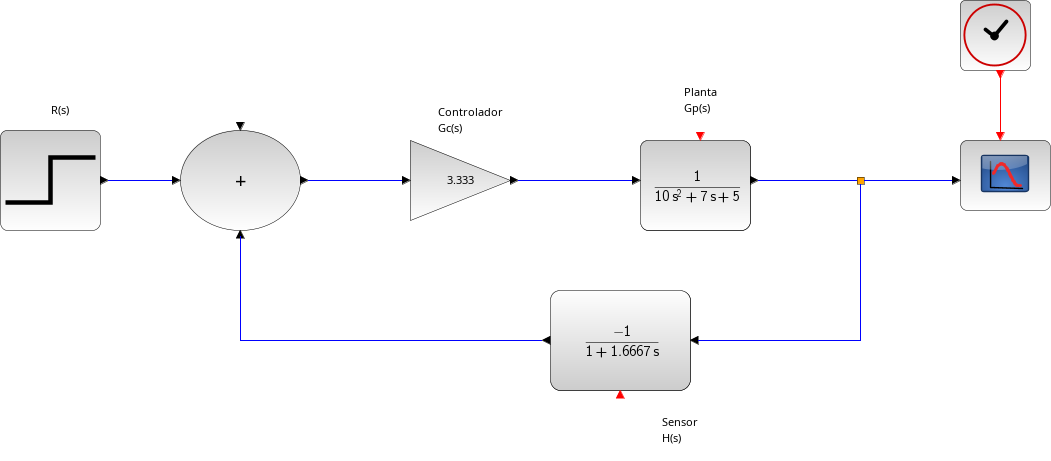
\includegraphics[width=0.8\textwidth]{atividades/4-atividade/assets/diagrama-blocos.png}
    \caption{Diagrama de blocos do sistema de controle proporcional.}
    \label{fig:diagrama_blocos}
\end{figure}

O diagrama de blocos apresentado na Figura~\ref{fig:diagrama_blocos} ilustra a configuração do sistema de controle:

\begin{itemize}
    \item \textbf{Controlador Proporcional (\(G_c(s)\))}: Com ganho de \(\frac{10}{3}\) = (\(3.333\)), o controlador ajusta a saída com base na diferença entre a referência e o sinal medido pelo sensor.
    \item \textbf{Planta (\(G_p(s)\))}: Representada pela função de transferência \(\frac{1}{10s^2 + 7s + 5}\), que descreve a dinâmica do sistema massa-mola-amortecedor.
    \item \textbf{Sensor (\(H(s)\))}: O sensor é modelado como um sistema de primeira ordem com a função de transferência \(\frac{1}{1 + 1.6667s}\), capturando a resposta da variável controlada com uma certa constante de tempo.
    \item \textbf{Soma (\(\Sigma\))}: Um somador que computa a diferença entre a referência e a saída do sensor, alimentando essa diferença para o controlador.
    \item \textbf{Feedback}: O loop de feedback é crucial para garantir que a saída do sistema esteja em conformidade com a entrada desejada.
\end{itemize}

O sistema é projetado para monitorar e ajustar a saída de modo a atingir um estado desejado, com foco na estabilidade e eficiência do controle.



% ===============================================================
% Letra B =======================================================
\subsection{Parte (b): Função de Transferência em Malha Fechada}

Para o sistema de controle proposto, primeiramente definimos os parâmetros físicos e as configurações do sistema. A planta é um sistema massa-mola-amortecedor, e o controlador utilizado é um controlador proporcional. O sensor é modelado por um sistema de primeira ordem. Os parâmetros são definidos como segue:

\begin{itemize}
    \item Massa, \(m = 10\, \text{kg}\)
    \item Coeficiente de amortecimento, \(c = 7\, \text{Ns/m}\)
    \item Constante da mola, \(k = 5\, \text{N/m}\)
\end{itemize}

O ganho do controlador proporcional, \(K\), é definido como:
\[ K = \frac{m}{3} \]

A constante de tempo do sensor, \(T_s\), é determinada por:
\[ T_s = \frac{m}{6} \]

As funções de transferência para a planta (\(G_p(s)\)), o sensor (\(H_s(s)\)), e o controlador proporcional (\(G_c(s)\)) são definidas da seguinte forma:
\begin{align*}
    G_p(s) & = \frac{1}{m s^2 + c s + k} = \frac{1}{10 s^2 + 7 s + 5} \\
    H_s(s) & = \frac{1}{T_s s + 1} = \frac{1}{\frac{10}{6} s + 1}     \\
    G_c(s) & = K = \frac{10}{3}
\end{align*}

\subsubsection{Código Scilab utilizado calcular a Função de Transferência em Malha Fechada}
\begin{lstlisting}[language=Scilab, caption=Código Scilab para calcular a função de transferência em malha fechada]
    // Definicao dos parametros
    s = poly(0, 's');
    m = 10;  // massa
    c = 7;   // coeficiente de amortecimento
    k = 5;   // constante da mola
    
    // Definicao das funcoes de transferencia
    K = m / 3;  // Ganho do controlador proporcional
    Ts = m / 6;  // Constante de tempo do sensor
    
    // Funcoes de Transferencia
    Gp = syslin('c', 1, m*s^2 + c*s + k);  // Planta
    Hs = syslin('c', 1, Ts*s + 1);  // Sensor
    Gc = syslin('c', K, 1);  // Controlador Proporcional
    
    // Funcao de Transferencia em Malha Fechada C(s)/R(s)
    sys = Gc * Gp / (1 + Gc * Gp * Hs);
    
    // Exibicao da Funcao de Transferencia em Malha Fechada
    disp("Funcao de Transferencia em Malha Fechada C(s)/R(s):");
    disp(sys);
    \end{lstlisting}



A função de transferência em malha fechada \(C(s)/R(s)\) é calculada pela integração dessas funções de transferência, resultando na seguinte expressão:
\[
    C(s)/R(s) = \frac{G_c(s) G_p(s)}{1 + G_c(s) G_p(s) H_s(s)}
\]

Após a simplificação e cálculos realizados pelo software Scilab, a função de transferência em malha fechada resultante é:
\[
    \frac{0.2 + 0.3333333s}{0.5 + 0.92s + 1.3s^2 + s^3}
\]

Esta função de transferência em malha fechada indica como o sistema responde à entrada \(R(s)\) dada a configuração de controle atual. A expressão mostra a relação entrada-saída considerando a realimentação do sensor e a ação do controlador proporcional.


% ===============================================================
% Letra C =======================================================

\subsection{Parte (c): Análise de Estabilidade com o Critério de Routh-Hurwitz}

Após calcular a função de transferência em malha fechada \(C(s)/R(s)\), o próximo passo é analisar a estabilidade do sistema de controle. Utilizamos o critério de Routh-Hurwitz para essa finalidade, que é uma técnica fundamental na teoria de controle para determinar a estabilidade de um sistema linear.


\subsubsection{Código Scilab para a Análise de Routh-Hurwitz}
\begin{lstlisting}[language=Scilab, caption=Código Scilab para calcular a matriz de Routh-Hurwitz]
    // Definicao dos parametros
    s = poly(0, 's');
    m = 10;  // massa
    c = 7;   // coeficiente de amortecimento
    k = 5;   // constante da mola

    // Definicao das funcoes de transferencia
    K = m / 3;  // Ganho do controlador proporcional
    Ts = m / 6;  // Constante de tempo do sensor

    // Funcoes de Transferencia
    Gp = syslin('c', 1, m*s^2 + c*s + k);  // Planta
    Hs = syslin('c', 1, Ts*s + 1);  // Sensor
    Gc = syslin('c', K, 1);  // Controlador Proporcional

    // Funcao de Transferencia em Malha Fechada C(s)/R(s)
    sys = Gc * Gp / (1 + Gc * Gp * Hs);

    // Extraindo o denominador da Funcao de Transferencia para Analise de Estabilidade
    den = sys.den;

    rh_matrix = routh_t(den);

    // Exibir a Matriz de Routh-Hurwitz
    disp("Matriz de Routh-Hurwitz:");
    disp(rh_matrix);
\end{lstlisting}


\subsubsection{Extração do Denominador da Função de Transferência}

A estabilidade de um sistema de controle pode ser analisada pelo estudo das raízes do polinômio característico do denominador da função de transferência em malha fechada. Estas raízes, também conhecidas como pólos do sistema, determinam como o sistema responde a diferentes entradas ao longo do tempo. A localização desses pólos no plano complexo indica se as respostas do sistema serão estáveis, instáveis ou em um estado de margem de estabilidade.

No caso do sistema considerado, a função de transferência em malha fechada resultante é calculada pelo produto e pela soma das funções de transferência do controlador proporcional, da planta e do sensor, estruturados como segue:
\[
    C(s)/R(s) = \frac{Gc \times Gp}{1 + Gc \times Gp \times Hs}
\]
A partir desta expressão, o denominador, que contém o polinômio característico do sistema, é dado por:
\[
    1 + Gc \times Gp \times Hs
\]
Expandindo e simplificando este produto usando os parâmetros e as funções definidas no código Scilab, o denominador da função de transferência em malha fechada é obtido. Este processo resulta em um polinômio em \(s\) que representa a combinação das dinâmicas do controlador, da planta e do sensor.

Para este sistema específico, utilizando os parâmetros dados, o denominador extraído e simplificado é:
\[
    0.5 + 0.92s + 1.3s^2 + s^3
\]
Este polinômio é então usado para a construção da matriz de Routh-Hurwitz, que é uma técnica clássica de análise de estabilidade, ajudando a determinar a presença de raízes com partes reais não negativas e, consequentemente, se o sistema é estável ou não.



\subsubsection{Cálculo da Matriz de Routh-Hurwitz}

Para construir a matriz de Routh-Hurwitz, utilizamos a função \texttt{routh\_t} que calcula essa matriz a partir do polinômio característico. A matriz de Routh-Hurwitz para o denominador do sistema é calculada e apresentada como segue:
\[
    \begin{array}{c|cc}
        s^3 & 1         & 0.92 \\
        s^2 & 1.3       & 0.5  \\
        s^1 & 0.5353846 & 0    \\
        s^0 & 0.5       &      \\
    \end{array}
\]

\subsubsection{Interpretação da Matriz de Routh-Hurwitz}

Os elementos da primeira coluna da matriz de Routh-Hurwitz indicam a estabilidade do sistema. Todos os elementos devem ser positivos para garantir estabilidade. A matriz mostra que todos os termos são positivos, sugerindo que o sistema é estável. Esta análise detalhada fornece confiança adicional na robustez do sistema sob a configuração de controle atual.

\subsubsection{Conclusão da Análise de Estabilidade}

A análise com a matriz de Routh-Hurwitz confirma que o sistema é estável sob as condições atuais. A positividade de todos os termos na primeira coluna da matriz assegura que não há raízes com partes reais positivas, o que implica em uma resposta do sistema estável e controlada. Essa conclusão é vital para garantir que o sistema opere de forma segura e eficaz, mantendo o desempenho desejado.

% ===============================================================
% Letra D =======================================================
\subsection{Parte (d): Análise de Estabilidade para Diferentes Valores de \(K\)}

A estabilidade do sistema de controle é investigada para uma variação do ganho \(K\) do controlador proporcional, substituído pelo parâmetro variável \(K\). Utilizamos a função de transferência em malha fechada definida pelos parâmetros físicos do sistema para determinar para quais valores de \(K\) o sistema é estável.

\subsubsection{Definição da Função de Transferência}
Com base nos parâmetros do sistema, a função de transferência da planta \(G_p(s)\) e do sensor \(H_s(s)\) são definidas como segue:

\[
    G_p(s) = \frac{1}{10 s^2 + 7 s + 5}
\]

\[
    H_s(s) = \frac{1}{\frac{10}{6} s + 1}
\]

\subsubsection{Função de Transferência em Malha Fechada}
A função de transferência em malha fechada \(T(s)\), considerando o controlador proporcional \(G_c(s) = K\), é dada por:

\[
    T(s) = \frac{K \cdot G_p(s)}{1 + K \cdot G_p(s) \cdot H_s(s)}
\]

Substituindo \(G_c(s)\), \(G_p(s)\), e \(H_s(s)\) com os valores acima, obtemos:

\[
    T(s) = \frac{K \left(\frac{1}{10 s^2 + 7 s + 5}\right)}{1 + K \left(\frac{1}{10 s^2 + 7 s + 5}\right) \left(\frac{1}{\frac{10}{6}s + 1}\right)}
\]

Multiplicando numerador e denominador pelo MMC dos denominadores das funções de transferência, obtemos:

\[
    T(s) = \frac{5Ks + 3K}{3K + 50s^3 + 65s^2 + 46s + 15}
\]
Esta função representa a resposta do sistema em função do ganho proporcional \(K\), onde \(K\) modula a entrada em função das dinâmicas combinadas da planta e do sensor.

\subsubsection{Construção da Matriz de Routh-Hurwitz}

A análise da estabilidade do sistema é feita através da matriz de Routh-Hurwitz, que é construída a partir do polinômio característico:
\[
    50s^3 + 65s^2 + 46s + 15 + 3K
\]

A estabilidade do sistema é analisada através da construção da matriz de Routh-Hurwitz para o polinômio característico derivado do denominador da função de transferência em malha fechada:
\[
    \begin{array}{c|cc}
        s^3 & 50                     & 46      \\
        s^2 & 65                     & 15 + 3K \\
        s^1 & \frac{150K - 2240}{65} & 0       \\
        s^0 & 15 + 3K                &         \\
    \end{array}
\]
Onde:
\[
    s^1 = \frac{150K - 2240}{65} = 2.3077K - 34.4615
\]

\subsubsection{Análise de Condições de Estabilidade}
Para garantir a estabilidade, todos os coeficientes na primeira coluna da matriz de Routh-Hurwitz devem ser positivos:
\begin{itemize}
    \item \(s^3 = 50\) é constantemente positivo.
    \item \(s^2 = 65\) é positivo.
    \item \(s^1 = 2.3077K - 34.4615 > 0\), o que requer que \(K\) seja menor que \(\frac{34.4615}{2.3077} \approx 14.93\) para manter a positividade deste termo. Assim, a estabilidade é assegurada para \(K < 14.93\).
    \item \(s^0 = 15 + 3K > 0\), que é trivialmente satisfeito desde que \(K > -5\), mas a condição mais restritiva vem de \(s^1\).
\end{itemize}

\subsubsection{Conclusão da Análise de Condições de Estabilidade}
A análise meticulosa da matriz de Routh-Hurwitz indica que o sistema mantém a estabilidade quando o ganho proporcional, \(K\), está dentro do intervalo especificado. Valores de \(K\) superiores a 14.93 podem induzir instabilidade, manifestando-se através de oscilações não amortecidas ou respostas exageradas a perturbações, comprometendo tanto a performance quanto a segurança operacional do sistema.

Assim, é fundamental que \(K\) seja cuidadosamente escolhido para manter-se dentro do intervalo \(0 < K < 14.93\) para assegurar um comportamento estável e previsível do sistema em todas as condições operacionais. % Completa e validada
\section{Atividade 5}

\subsection{Descrição do Modelo e Simulação}
Nesta atividade, simulamos um sistema de controle que envolve um sistema massa-mola-amortecedor com um controlador proporcional. O sistema é descrito pela seguinte equação diferencial:
\[
    m\frac{d^2x(t)}{dt^2} + c\frac{dx(t)}{dt} + kx(t) = f(t),
\]
onde \( m = 10 \), \( c = 7 \), e \( k = 5 \).

\subsection{Construção do Diagrama de Blocos}
O diagrama dde blocos para o sistema é apresentado a seguir, ilustrando como os componentes do sistema — controlador, planta e sensor — estão interligados.

\begin{figure}[H]
    \centering
    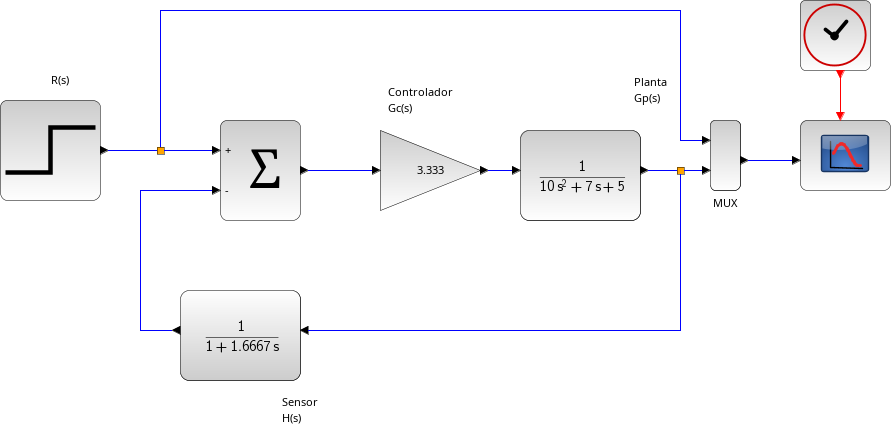
\includegraphics[width=0.7\textwidth]{atividades/5-atividade/assets/diagrama-a.png}
    \caption{Diagrama de blocos do sistema de controle para Atividade 5}
    \label{fig:diagrama_blocos_5}
\end{figure}

\subsection{Simulação do Sistema}
Para a simulação, utilizamos um sinal de degrau com amplitude \( A = \frac{m}{4} = 2.5 \). O tempo de simulação foi definido em 50 segundos para permitir a observação completa da resposta do sistema.

\subsubsection{Configuração da Simulação}
O sinal de degrau foi configurado para iniciar em 0 e atingir 2.5 no instante \( t = 1 \) segundo. O tempo de simulação total foi estabelecido para 50 segundos para assegurar que a resposta do sistema fosse completamente observada.

\begin{figure}[H]
    \centering
    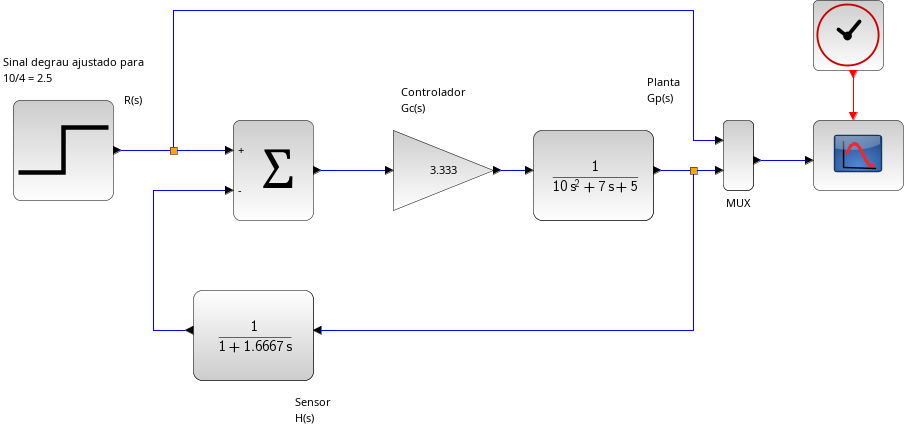
\includegraphics[width=0.8\textwidth]{atividades/5-atividade/assets/diagrama-b.png}
    \caption{Diagrama de blocos utilizado para a simulação}
    \label{fig:diagrama_blocos_b}
\end{figure}
\subsubsection{Resultados da Simulação}
A resposta do sistema ao degrau é apresentada na figura abaixo, onde são destacados o tempo de subida, tempo de pico, tempo de acomodação e a zona estacionária, utilizando a ferramenta DataTip para marcar esses pontos significativos.

\begin{figure}[H]
    \centering
    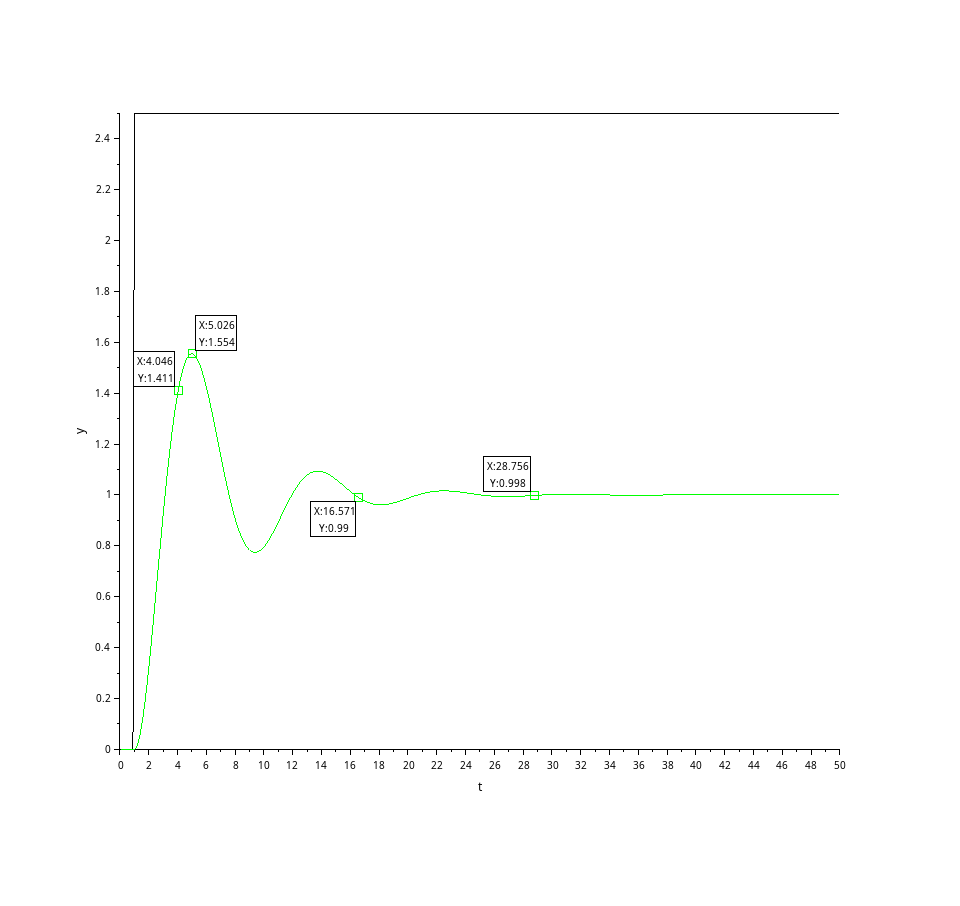
\includegraphics[height=0.7\textwidth]{atividades/5-atividade/assets/simulation-b.png}
    \caption{Resposta do sistema ao degrau com configuração de amplitude \( A = 2.5 \)}
    \label{fig:simulation_5b}
\end{figure}

\subsection{Análise Detalhada dos Resultados da Simulação}
A resposta do sistema ao degrau é apresentada na Figura \ref{fig:simulation_5b}, demonstrando as dinâmicas chave do sistema controlado. Analisamos detalhadamente cada parte da resposta:

\begin{itemize}
    \item \textbf{Tempo de Subida:} O tempo de subida refere-se ao intervalo necessário para que a resposta do sistema suba do estado inicial até um determinado percentual do valor final, geralmente 90\%. No gráfico, o sistema leva aproximadamente 4.8 segundos para atingir um valor próximo de 1.55, que é o primeiro pico significativo. Este comportamento inicial mostra como o sistema responde rapidamente ao degrau, com a energia inicialmente absorvida e depois liberada pela combinação de massa, mola e amortecedor.
    \item \textbf{Tempo de Pico:} O pico ocorre no momento em que a saída atinge seu valor máximo em resposta ao degrau. O primeiro pico de 1.55 é atingido em torno de 5 segundos após a aplicação do degrau, ilustrando a máxima extensão da resposta do sistema antes de começar a amortecer devido às forças de fricção e à força restauradora da mola.

    \item \textbf{Tempo de Acomodação:} Após o pico inicial, o sistema começa a se estabilizar, reduzindo as oscilações até alcançar um estado quase constante. Este período é crucial, pois mostra a eficácia do amortecimento em dissipar a energia inicialmente induzida. No gráfico, o sistema mostra sinais de acomodação em torno de 28 segundos, indicando que o amortecimento e a rigidez da mola estão bem dimensionados para controlar as oscilações.

    \item \textbf{Zona Estacionária:} O sistema é considerado em estado estacionário quando as oscilações em torno do valor de equilíbrio se tornam negligíveis. No gráfico, isso é observado após aproximadamente 28 segundos, onde a saída mantém-se constante em cerca de 0.998. Esta fase é fundamental para avaliar se o sistema atingiu o equilíbrio desejado após a perturbação inicial.
\end{itemize}


\textbf{Conclusões da Análise:} A resposta ao degrau revela que o sistema massa-mola-amortecedor, equipado com um controlador proporcional, consegue retornar a um estado de equilíbrio após uma perturbação inicial. A análise destaca a importância de um ajuste apropriado do amortecimento e da rigidez da mola para assegurar que o sistema não apenas retorne ao equilíbrio, mas que o faça de maneira eficiente e sem oscilações excessivas. Este comportamento é indicativo de um sistema bem projetado, capaz de manter a estabilidade mesmo sob condições iniciais desafiadoras.


\subsection{Simulação com Diferentes Configurações de Ganho e Amplitude}
Nesta seção, expandimos a simulação para avaliar o impacto de diferentes configurações de ganho do controlador e amplitude do sinal de entrada. Três casos distintos foram simulados:


\begin{enumerate}
    \item \textbf{Caso Base (Amplitude A=1, Ganho=3.333)}: Mostrado pela linha verde no gráfico.
    \item \textbf{Caso com A=2.5 e Ganho=3.333}: Mostrado pela linha amarela no gráfico.
    \item \textbf{Caso com A=2.5 e Ganho=6.666}: Mostrado pela linha azul no gráfico.
\end{enumerate}

\begin{figure}[H]
    \centering
    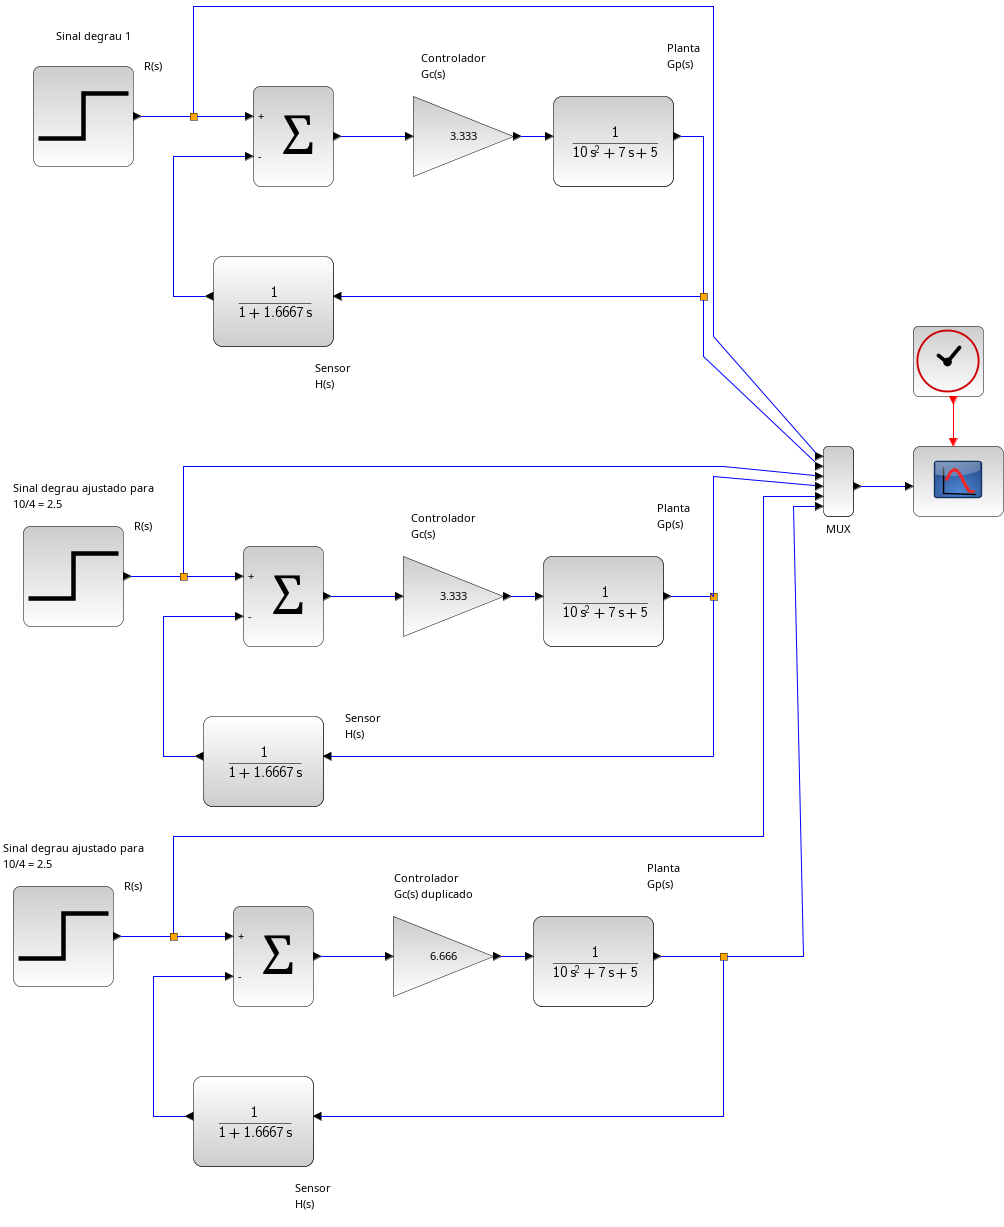
\includegraphics[width=0.8\textwidth]{atividades/5-atividade/assets/diagrama-c.png}
    \caption{Diagrama de blocos utilizado para a simulação dos três casos}
    \label{fig:diagrama_blocos_c}
\end{figure}

\subsubsection{Análise dos Resultados}
Os resultados das simulações são visualizados no gráfico seguinte, onde diferentes cores representam os diferentes casos testados.



\begin{figure}[H]
    \centering
    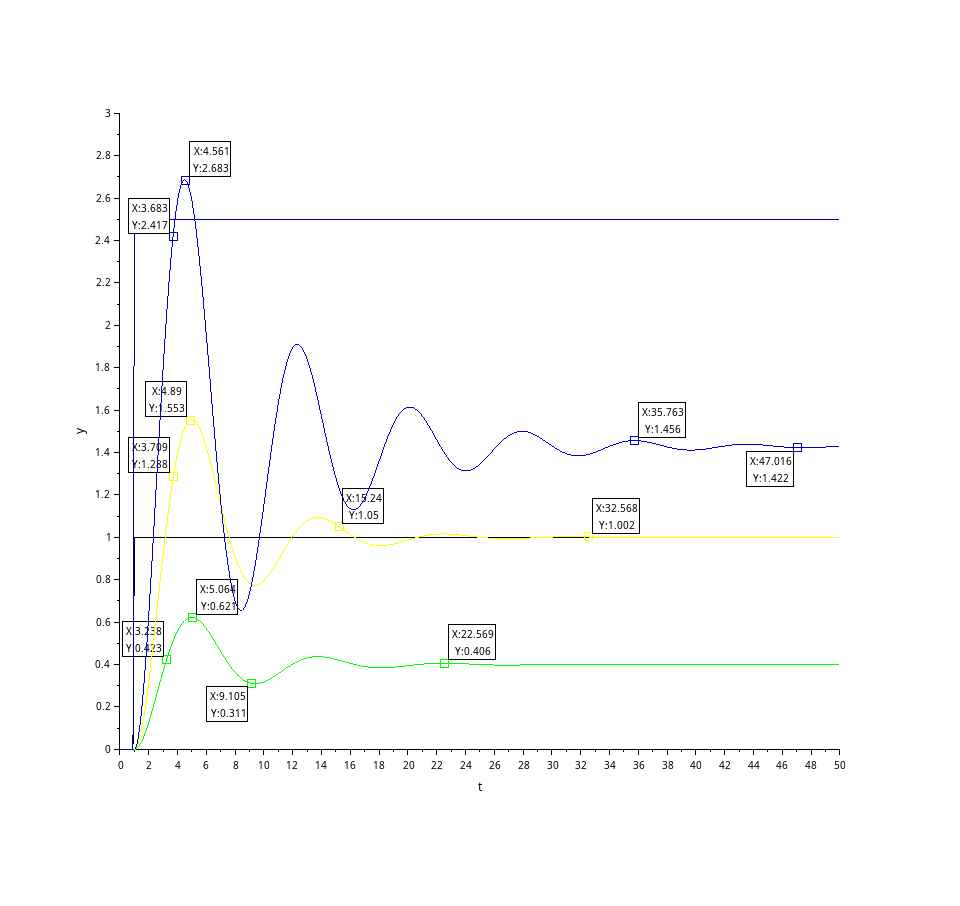
\includegraphics[width=0.8\textwidth]{atividades/5-atividade/assets/simulation-c.png}
    \caption{Resposta do sistema para diferentes configurações de ganho e amplitude}
    \label{fig:response_comparison}
\end{figure}

\begin{itemize}
    \item \textbf{Verde (Caso Base)}: A resposta é bastante atenuada, com um pico máximo de aproximadamente 0.311 e acomodação rápida. Este caso mostra a capacidade do sistema de controlar eficazmente pequena perturbações.

    \item \textbf{Amarelo (A=2.5, Ganho=3.333)}: Com o aumento da amplitude, o sistema apresenta um overshoot maior, atingindo aproximadamente 1.554, com oscilações mais pronunciadas antes de estabilizar perto de 1.002. Isso indica que a resposta é mais vigorosa devido à maior entrada, mas ainda gerenciável.

    \item \textbf{Azul (A=2.5, Ganho=6.666)}: O aumento do ganho resulta em um overshoot significativamente maior, cerca de 2.683, com oscilações prolongadas que se estendem ao longo de todo o período de simulação. A resposta é mais agressiva e menos estável, demonstrando que um ganho mais alto pode introduzir instabilidade no sistema.
\end{itemize}

\subsection{Comparação e Comentários sobre as Respostas}
A comparação entre os três casos ilustra claramente a influência da amplitude do sinal de entrada e do ganho do controlador sobre a dinâmica do sistema. As principais observações são:

\begin{itemize}
    \item \textbf{Impacto do Aumento da Amplitude}: O aumento da amplitude do degrau de 1 para 2.5 resulta em um maior overshoot e tempo de acomodação mais longo, o que é esperado em sistemas de controle devido à maior energia introduzida no sistema.

    \item \textbf{Efeitos do Aumento do Ganho do Controlador}: Ao dobrar o ganho do controlador de 3.333 para 6.666, enquanto mantendo a amplitude elevada, observa-se uma resposta muito mais volátil e um pico de overshoot quase dobrado. Isso sugere que embora um ganho mais alto possa ser benéfico para uma resposta mais rápida, também pode comprometer a estabilidade geral do sistema.

    \item \textbf{Conclusões}: Os resultados indicam que um ajuste cuidadoso do ganho é crucial, especialmente em sistemas onde a estabilidade é uma preocupação. Para aplicações que requerem respostas rápidas e podem tolerar algum overshoot, um ganho mais alto pode ser apropriado. No entanto, para a maioria das aplicações industriais e comerciais, um ganho mais moderado e uma abordagem balanceada são recomendados para evitar oscilações excessivas e garantir a estabilidade do sistema.
\end{itemize}

Conclusivamente, esta análise demonstra a importância de um design de controlador bem ponderado, ressaltando a necessidade de equilibrar resposta rápida e estabilidade, dependendo dos requisitos específicos da aplicação.
 % Completa e validada

\section{Atividade 6}

\subsection{Introdução ao Modelo com Controlador PID}
Os controladores PID são amplamente reconhecidos por sua eficácia e flexibilidade, combinando três elementos distintos para obter um desempenho superior: proporcional, integral e derivativo. Ao contrário dos controladores proporcionais, que ajustam a resposta do sistema de maneira direta ao erro atual, os controladores PID aproveitam três abordagens diferentes, cada uma desempenhando uma função específica.

O componente proporcional funciona de modo semelhante ao controlador proporcional simples, ajustando a saída do sistema em relação direta ao erro, com o objetivo de reduzir a diferença entre o valor medido e o valor desejado. No entanto, quando o componente proporcional sozinho não consegue corrigir totalmente o erro acumulado, entra em ação o componente integral, que soma e integra o erro ao longo do tempo para eliminá-lo.

Além disso, o componente derivativo desempenha um papel crucial ao prever mudanças no erro, ajudando a evitar que essas variações causem impactos negativos na saída do sistema. Com a integração desses três elementos, os controladores PID conseguem oferecer um controle mais preciso e estável, ajustando continuamente a saída para manter o sistema no estado desejado.
A fórmula padrão de um controlador PID pode ser representada pela equação \ref{eq:pid}:
\begin{equation}
    u(t) = K_p e(t) + K_i \int_{0}^{t} e(T) dT + K_d \frac{d e(t)}{dt}
    \label{eq:pid}
\end{equation}

O método de Ziegler-Nichols, desenvolvido por John G. Ziegler e Nathaniel B. Nichols, é uma técnica consolidada para a sintonia de controladores PID. Este método é particularmente útil porque simplifica a configuração dos controladores ao fornecer fórmulas práticas para calcular os ganhos \( K_p \), \( K_i \), e \( K_d \) com base na resposta do sistema a uma entrada de teste. Esses parâmetros são ajustados para otimizar a resposta do sistema em termos de tempo de subida, sobreposição e tempo de assentamento.

Os valores dos ganhos são estabelecidos de acordo com a estabilidade observada do sistema e são tipicamente calculados a partir do ganho crítico \( K_c \) e do período crítico \( P_c \), que são obtidos através de testes de malha aberta. A Tabela \ref{tab:ziegler-nichols} resume os valores recomendados para cada tipo de ganho:

\begin{table}[h]
    \centering
    \begin{tabular}{ccc}
        \hline
        \( K_p \)            & \( K_i \)                      & \( K_d \)              \\
        \hline
        \( 0,6 \times K_c \) & \( \frac{2}{P_c} \) & \( 0,125 \times P_c \) \\
        \hline
    \end{tabular}
    \caption{Valores dos ganhos segundo o método de Ziegler-Nichols}
    \label{tab:ziegler-nichols}
\end{table}

% ===============================================================
% Letra A Validado ==============================================
\subsection{Controlador PID}

Com base nas análises conduzidas na Atividade 4, foi estabelecido um valor limite para o ganho crítico, \( K_c \), de 14.93. Este parâmetro é crucial para o ajuste dos parâmetros do controlador PID utilizando o método de Ziegler-Nichols. Semelhante ao procedimento adotado na Atividade 5, simulou-se o comportamento do sistema com um sinal de entrada em forma de degrau, cuja amplitude é definida como \( A = \frac{m}{4} \). Considerando que \( m = 10 \), a amplitude do degrau é \( A = 2.5 \). Este cenário permitiu a observação direta das respostas do sistema sob o efeito do ganho crítico.

\begin{figure}[H]
    \centering
    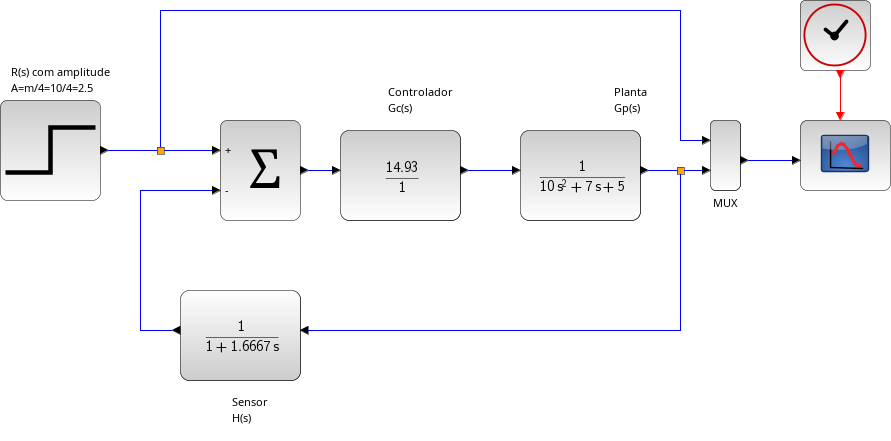
\includegraphics[width=0.7\textwidth]{atividades/6-atividade/assets/a/diagrama-ganho-critico-sistema-instavel.png}
    \caption{Diagrama mostrando o sistema no ponto crítico com \( K_c = 14.93 \)}
    \label{fig:diagrama-ponto-critico}
\end{figure}

A simulação realizada no ganho crítico, \( K_c = 14.93 \), demonstra que o sistema atinge uma condição de oscilação não amortecida, o que é indicativo de uma fronteira entre a estabilidade e a instabilidade. Essa observação é fundamental, pois o ponto de oscilação não amortecida é usado pelo método de Ziegler-Nichols para calibrar os controladores PID, visando uma resposta rápida e minimamente oscilatória em regime permanente.

\begin{figure}[H]
    \centering
    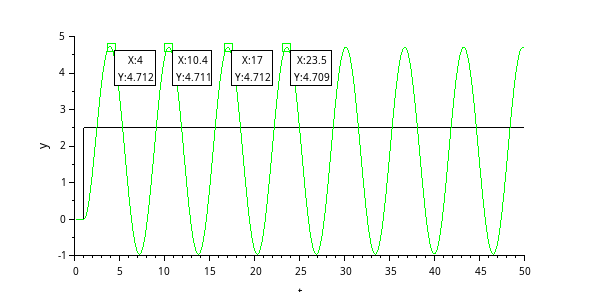
\includegraphics[width=0.7\textwidth]{atividades/6-atividade/assets/a/ganho-critico-sistema-instavel.png}
    \caption{Resposta do sistema com o controlador PID ajustado para \( K_c = 14.93 \)}
    \label{fig:ganho-critico-sistema-instavel}
\end{figure}


Como observado no gráfico de resposta temporal, o sistema exibe oscilações contínuas com uma amplitude aproximadamente constante, confirmando a caracterização do ganho crítico. Esta condição é explorada para determinar o período crítico \( P_c \), calculado pela medição do intervalo entre picos consecutivos. O valor de \( P_c \) é crucial para definir os parâmetros do controlador PID, pois influencia diretamente a dinâmica de correção implementada pelo controlador.

Os dados obtidos deste experimento são essenciais para a calibração dos parâmetros do controlador PID. Ajustar o controlador para operar próximo do ponto crítico, mas com garantias de estabilidade, permite aproveitar a máxima capacidade de resposta do sistema sem comprometer sua segurança operacional. Esta abordagem visa melhorar tanto a eficiência quanto a estabilidade do sistema, tornando o controle mais robusto frente a variações nas condições operacionais.

\subsubsection{Determinação do Período Crítico}
O período crítico \( P_c \) foi determinado a partir da análise do gráfico de resposta em regime oscilatório no ganho crítico. Identificamos os picos consecutivos e medimos o tempo entre eles para calcular o \( P_c \). A partir dos pontos identificados no gráfico, com os tempos \( t_1 = 9.98 \, \text{s} \) e \( t_2 = 16.894 \, \text{s} \), o período crítico foi calculado como:
\[
    P_c = t_2 - t_1 = 16.894 - 9.98 = 6.914 \, \text{s}
\]
Este valor é importante para o ajuste subsequente dos parâmetros do controlador PID utilizando o método de Ziegler-Nichols.


\subsubsection{Determinação dos Parâmetros do Controlador PID}
Após identificarmos o ganho crítico \( K_c = 14.93 \) através de análises detalhadas, empregamos o método de Ziegler-Nichols para ajustar os parâmetros do controlador PID. Este método é eficaz para sintonizar controladores em sistemas onde a resposta precisa ser otimizada em termos de estabilidade e rapidez.

\subsubsection{Cálculo dos Parâmetros do Controlador PID}
O método de Ziegler-Nichols, conhecido por sua eficiência na configuração inicial de controladores PID, utiliza o ganho crítico \( K_c \) e o período crítico \( P_c \) para estabelecer os parâmetros de controle, ajustando assim a resposta do sistema.

\begin{itemize}
    \item \textbf{Ganho Proporcional} \( K_p \):
          \[
              K_p = 0.6 \times K_c = 0.6 \times 14.93 = 8.958
          \]
    \item \textbf{Ganho Integral} \( K_i \):
          \[
              K_i = \frac{2}{P_c} = \frac{2}{6.914} \approx 0.289
          \]
    \item \textbf{Ganho Derivativo} \( K_d \):
          \[
              K_d = 0.125 \times P_c = 0.125 \times 6.914 = 0.864
          \]
\end{itemize}

\subsubsection{Implementação e Validação dos Parâmetros}
Os parâmetros \( K_p = 8.958 \), \( K_i = 0.289 \), e \( K_d = 0.864 \) são implementados no controlador PID no ambiente de simulação Scilab. Esses valores são projetados para ajustar o sistema a fim de responder de forma ideal em diversas condições operacionais, melhorando tanto a estabilidade quanto a precisão do sistema.

A eficácia desses parâmetros será validada por meio de simulações adicionais, que irão confirmar se eles conseguem manter o desempenho desejado do sistema, assegurando que o controle PID seja eficiente e eficaz.

\begin{figure}[H]
    \centering
    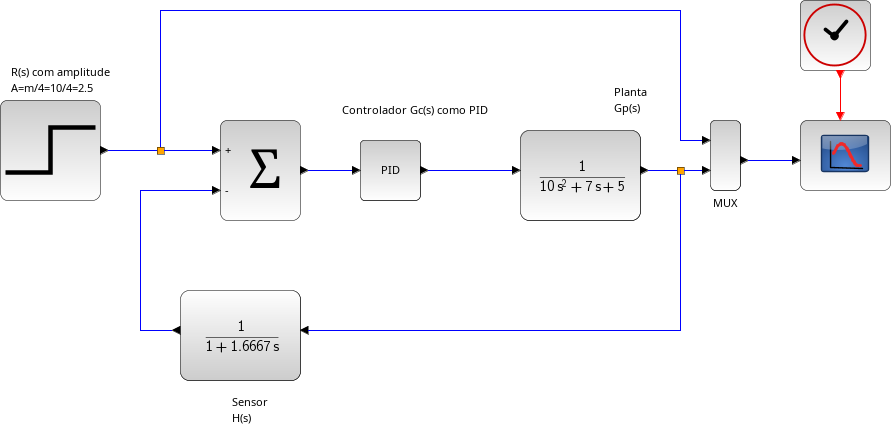
\includegraphics[width=0.8\textwidth]{atividades/6-atividade/assets/a/diagrama-pid.png}
    \caption{Resposta do sistema com os parâmetros do PID ajustados.}
    \label{fig:diagrama-pid}
\end{figure}

\begin{figure}[H]
    \centering
    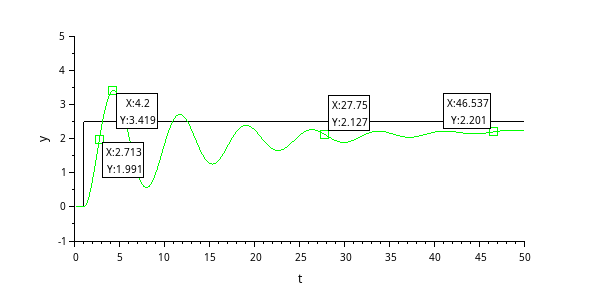
\includegraphics[width=0.8\textwidth]{atividades/6-atividade/assets/a/pid.png}
    \caption{Resposta do sistema com os parâmetros do PID ajustados.}
    \label{fig:resposta-pid}
\end{figure}

Após a validação inicial, pode ser necessário um refinamento manual dos parâmetros para otimizar ainda mais a resposta do sistema. Este processo de ajuste fino baseia-se na análise detalhada das respostas obtidas e na experiência prática, permitindo uma sintonia mais precisa que se adapta adequadamente às especificidades do sistema e às variações nas condições operacionais. Este ajuste é crucial para alcançar o melhor equilíbrio entre estabilidade e rapidez na resposta do controlador PID.

Subsequentemente, novas simulações serão realizadas para validar a eficácia dos parâmetros ajustados. Esta etapa é fundamental para verificar se os ajustes refinados mantêm a saída do sistema próxima ao valor desejado sob uma gama mais ampla de condições operacionais, garantindo a eficácia e a eficiência do controle.

% ===============================================================
% Letra B Validado ==============================================
\subsection{Análise de Resposta com Controlador Proporcional e PID Ajustado}

Esta seção compara a resposta do sistema utilizando um controlador proporcional e um controlador PID ajustado, especificamente configurados com os parâmetros \( K_p = 8.958 \), \( K_i = 0.310 \), e \( K_d = 0.805 \). A análise foca na eficácia de cada controlador em atingir e manter o valor de referência desejado, sob uma amplitude de degrau de \( A = 2.5 \). Este estudo visa elucidar as vantagens e limitações de cada abordagem de controle em termos de resposta dinâmica e estabilidade.

\begin{figure}[H]
    \centering
    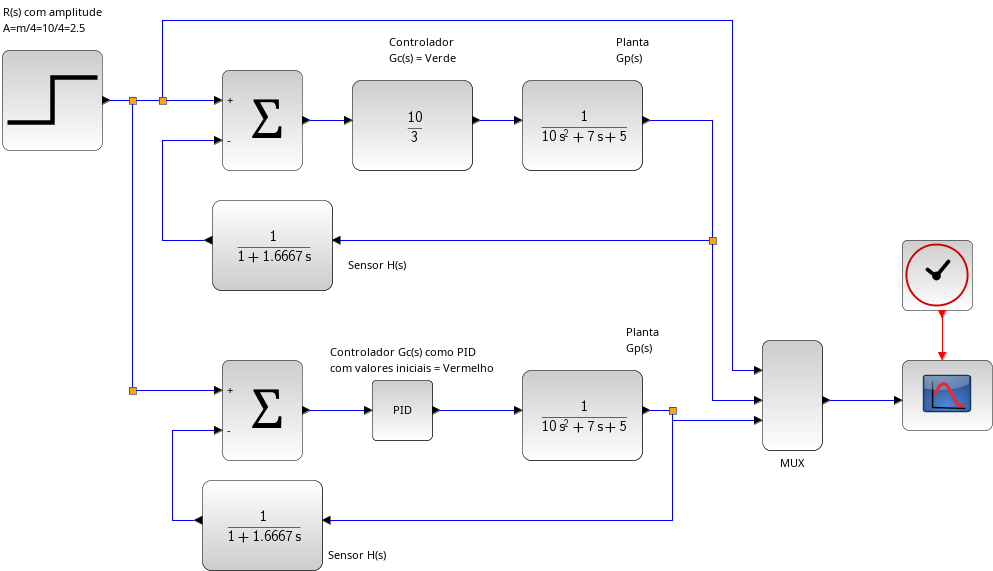
\includegraphics[width=0.8\textwidth]{atividades/6-atividade/assets/b/diagrama-comparacao-proporcional-pid.png}
    \caption{Diagrama ilustrativo do sistema de controle comparando a resposta com controlador proporcional e PID ajustado.}
    \label{fig:diagrama-comparacao-proporcional-pid}
\end{figure}

\begin{figure}[H]
    \centering
    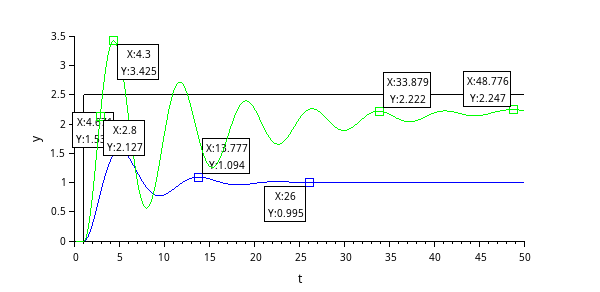
\includegraphics[width=0.8\textwidth]{atividades/6-atividade/assets/b/comparacao-proporcional-pid.png}
    \caption{Resposta temporal do sistema com controlador proporcional e PID ajustado.}
    \label{fig:comparacao-proporcional-pid}
\end{figure}

\subsubsection{Controlador Proporcional (Cor Azul)}
\textbf{Comportamento:}
O controlador proporcional oferece uma resposta imediata, característica desejada em muitas aplicações industriais por sua simplicidade e eficácia em sistemas menos complexos. No entanto, como evidenciado na Figura \ref{fig:comparacao-proporcional-pid}, ele falha em eliminar o erro de estado estacionário, estabilizando abaixo do valor de referência desejado.

\textbf{Estado Estacionário:}
A incapacidade de ajustar o erro estacionário torna o controlador proporcional menos adequado para aplicações que demandam precisão contínua e ajuste fino, pois não pode corrigir desvios permanentes sem intervenção externa.

\subsubsection{Controlador PID Ajustado (Cor Verde)}
\textbf{Comportamento:}
A configuração ajustada do PID demonstra superioridade em alcançar e manter o valor desejado rapidamente, com uma oscilação inicial (overshoot) significativamente reduzida e rápida estabilização, como ilustrado na Figura \ref{fig:comparacao-proporcional-pid}. Essa resposta é crucial em processos que não podem tolerar grandes desvios temporários ou onde o controle preciso é crítico.

\textbf{Estado Estacionário:}
O controlador PID, ajustado com parâmetros otimizados, mantém o valor de referência com alta precisão, ilustrando a importância da ação integral em corrigir erros acumulados e a ação derivativa em antecipar e mitigar futuras variações, resultando em uma resposta estável e precisa.

\subsubsection{Conclusão}
A análise comparativa entre o controlador proporcional e o PID ajustado destaca a simplicidade e a resposta imediata do primeiro, ideal para aplicações menos críticas, contra a precisão e a estabilidade superior do segundo. Com parâmetros ajustados (\(K_p = 8.958\), \(K_i = 0.310462589\), \(K_d = 0.80525\)), o controlador PID se adapta melhor às necessidades de aplicações que exigem controle dinâmico e alta fidelidade.

No entanto, é crucial reconhecer que os ajustes nos parâmetros \(K_p\), \(K_i\), e \(K_d\) do PID não são sem riscos e devem ser continuamente revisados. Alterações imprudentes em \(K_p\) podem levar a overshoots excessivos e instabilidade, enquanto \(K_i\) elevado pode causar oscilações indesejadas e resposta lenta, afetando negativamente a eficácia do sistema. Ajustes em \(K_d\) também requerem cautela, pois, embora possam melhorar a estabilidade, podem resultar em uma resposta demasiadamente amortecida.

Portanto, é recomendado que os ajustes nos parâmetros do PID sejam feitos com base em testes rigorosos e análise cuidadosa. A busca por um equilíbrio ótimo entre rapidez de resposta, estabilidade e precisão deve ser uma prática regular, adaptando o controlador às variações nas condições operacionais e às exigências específicas de cada aplicação. Esse processo contínuo de otimização ajuda a assegurar a performance aprimorada e a segurança do sistema controlado.


% ===============================================================
% Letra C Validado ==============================================
\subsection{Teste de Ajuste de Parâmetros do \( K_p \) do Controlador PID}

\subsubsection{Contextualização e Análise do Ajuste de \( K_p \)}
Para otimizar o desempenho do controlador PID, realizamos uma série de simulações alterando o valor de \( K_p \) para entender seu impacto na dinâmica do sistema. O objetivo foi encontrar um equilíbrio ideal entre a resposta rápida e a estabilidade do sistema, testando \( K_p \) em 80\% e 150\% do valor inicial de 8.958, além do próprio valor inicial.

\begin{figure}[H]
    \centering
    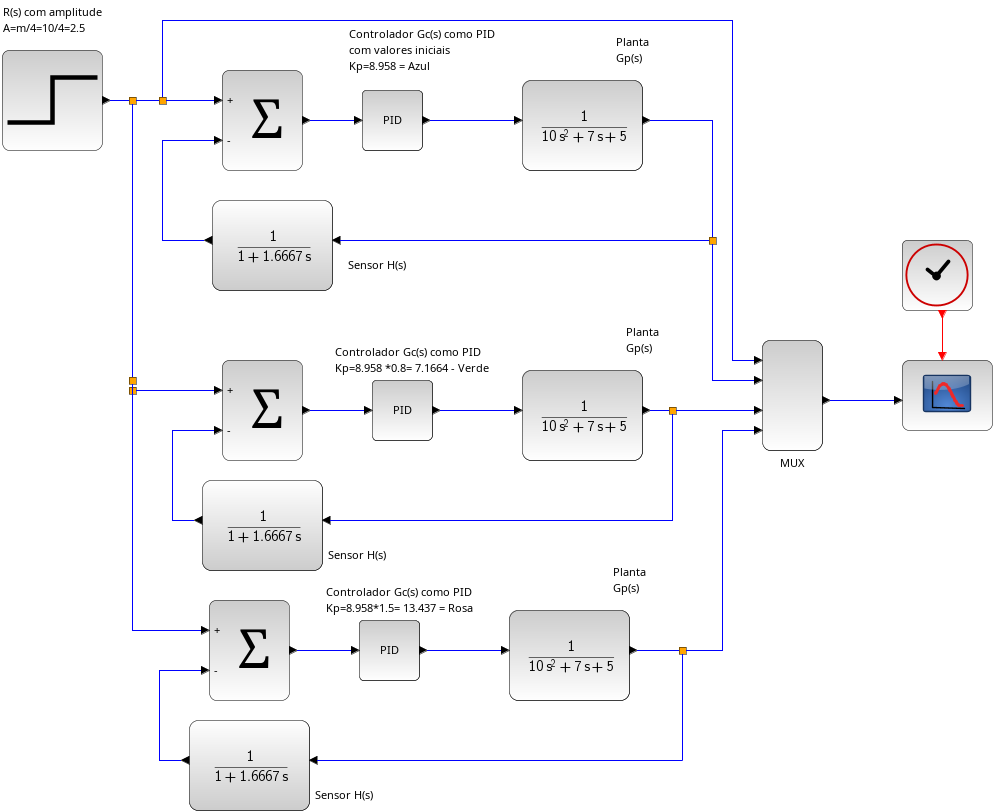
\includegraphics[width=0.8\textwidth]{atividades/6-atividade/assets/c/diagrama-pid-ajustando-kp.png}
    \caption{Diagrama de resposta do sistema com diferentes valores de \( K_p \).}
    \label{fig:diagrama-comparacao-proporcional-pid}
\end{figure}

\begin{figure}[H]
    \centering
    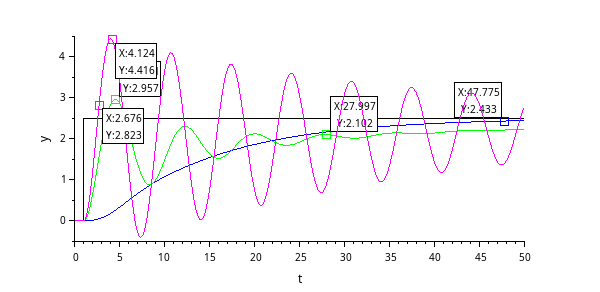
\includegraphics[width=0.8\textwidth]{atividades/6-atividade/assets/c/pid-ajustando-kp.png}
    \caption{Resposta do sistema para o \( K_p \) ajustado em comparação com outros valores.}
    \label{fig:comparacao-proporcional-pid}
\end{figure}

\subsubsection{Discussão dos Resultados e Escolha de \( K_p \)}
A análise das respostas mostrou que a redução de \( K_p \) para 7.1664 (80\% do valor inicial) oferece uma melhoria significativa em termos de controle de overshoot e estabilidade do sistema. Este ajuste resulta em uma resposta onde o overshoot é notavelmente menor, o que é vantajoso para sistemas que requerem estabilidade rápida sem oscilações excessivas.

\vspace{0.4cm}
\textbf{Vantagens:}
\begin{itemize}
    \item \textbf{Menor Overshoot:} Redução significativa no overshoot, proporcionando uma resposta mais suave e estável. Essa característica é particularmente benéfica para aplicações que não podem tolerar grandes desvios temporários de suas variáveis de processo.
    \item \textbf{Tempo de Acomodação Razoável:} O sistema atinge o estado estacionário mais rapidamente, o que é crucial para aplicações que demandam respostas rápidas e precisas. Isso é conseguido sem induzir instabilidade prolongada.
\end{itemize}

\vspace{0.4cm}
\textbf{Desvantagens:}
\begin{itemize}
    \item \textbf{Comprometimento da Rapidez Inicial:} A resposta inicial é ligeiramente mais lenta, o que pode não ser ideal para todos os tipos de aplicações, especialmente aquelas que dependem de uma atuação rápida após uma mudança de condições.
    \item \textbf{Sensibilidade a Distúrbios:} A redução do \( K_p \) pode diminuir a capacidade do sistema de reagir eficientemente a perturbações súbitas ou variações significativas na entrada, podendo resultar em um desempenho subótimo sob condições de carga variável.
\end{itemize}

Foi analisado da possibilidade de redução adicional de \( K_p \) diminuir ainda mais \( K_p \) além de 80\% poderia potencialmente levar a uma resposta demasiadamente lenta, comprometendo a capacidade do sistema de reagir a alterações rápidas. Essa mudança requer uma análise cuidadosa das prioridades do sistema: estabilidade versus rapidez de resposta.

\subsubsection{Implementação e Avaliação Futura do Novo \( K_p \)}
O novo \( K_p \) de 7.1664 será implementado no controlador PID para uso continuado. Este ajuste será acompanhado de monitoramento e avaliação contínuos para assegurar que ele atende às exigências do sistema em variadas condições operacionais.

A decisão de ajustar o \( K_p \) para 7.1664 reflete um compromisso bem fundamentado entre resposta rápida e controle de oscilações, adequado para muitas aplicações industriais e de automação. Avaliações futuras focarão em refinamentos adicionais e na otimização de \( K_i \) e \( K_d \) para maximizar a eficácia do sistema de controle.


% ===============================================================
% Letra D Validado ==============================================
\subsection{Comparação entre Controlador Proporcional, PID com Dados Iniciais e PID Ajustado}
Esta seção apresenta uma análise comparativa do desempenho de três configurações distintas de controladores: Proporcional, PID com valores iniciais e PID ajustado. A análise foca na resposta dos controladores em termos de estabilidade, tempo de resposta e precisão no estado estacionário. Ajustar o parâmetro \(K_p\) tem implicações significativas na dinâmica de controle, impactando diretamente a eficácia e eficiência do sistema.

\begin{figure}[H]
    \centering
    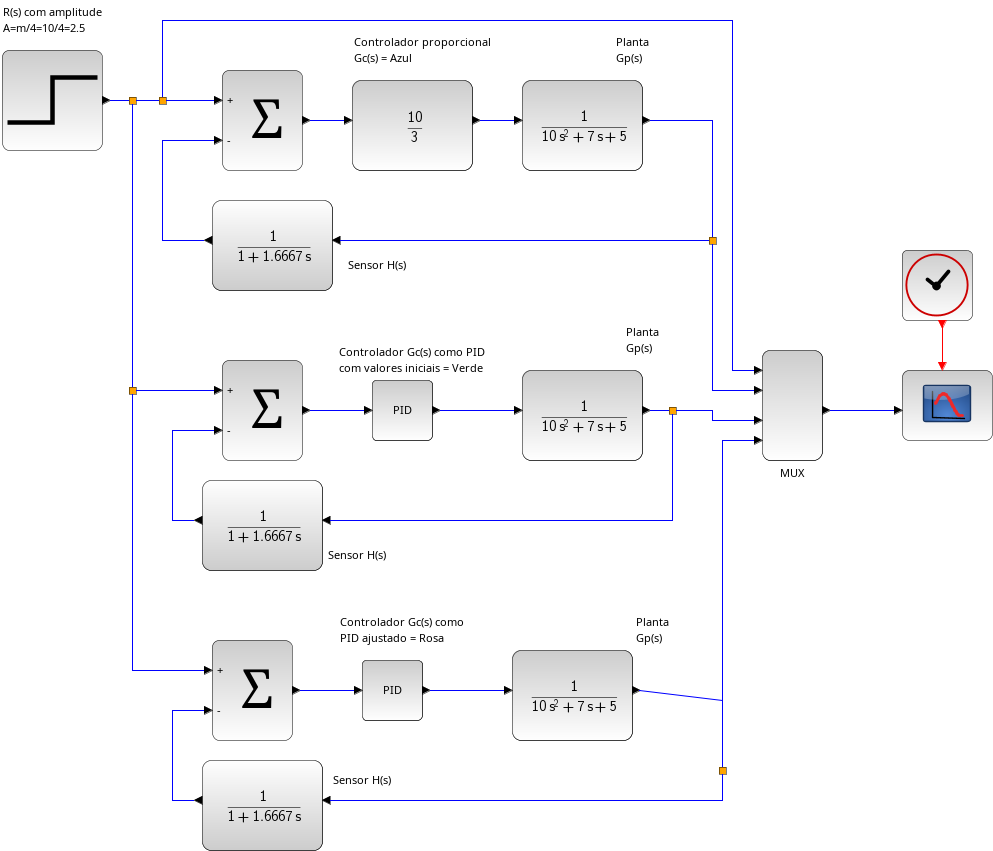
\includegraphics[width=0.8\textwidth]{atividades/6-atividade/assets/d/diagrama-comparacao-proporcional-pid-pid-ajustado.png}
    \caption{Diagrama de resposta do sistema com diferentes configurações de \(K_p\).}
    \label{fig:diagrama-comparacao-proporcional-pid-pid-ajustado}
\end{figure}

\begin{figure}[H]
    \centering
    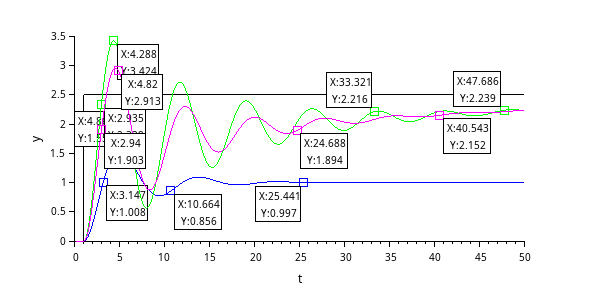
\includegraphics[width=0.8\textwidth]{atividades/6-atividade/assets/d/comparacao-proporcional-pid-pid-ajustado.png}
    \caption{Comparação das respostas temporais dos controladores sob a mesma condição de teste.}
    \label{fig:comparacao-proporcional-pid-pid-ajustado}
\end{figure}


\subsubsection{Análise dos Controladores}

\subsubsection{Controlador Proporcional (Cor Azul)}
\textbf{Comportamento:} O controlador proporcional, adequado para sistemas onde precisão extrema não é primordial, mostra uma resposta rápida inicial, mas falha em eliminar o erro de estado estacionário, uma limitação comum devido à ausência de ação integral.
\textbf{Estado Estacionário:} A resposta estabiliza significativamente abaixo do valor de referência, evidenciando a limitação deste tipo de controlador em corrigir completamente o erro de estado estacionário, adequado para aplicações onde desvios menores são toleráveis.

\subsubsection{PID com Valores Iniciais (Cor Verde)}
\textbf{Comportamento:} Este controlador exibe um overshoot inicial significativo e oscilações antes de estabilizar, característica de uma resposta rápida seguida de uma correção intensa pela ação integral.
\textbf{Estado Estacionário:} Atinge e mantém o valor desejado, com a componente integral ajustando o erro acumulado e garantindo que a saída final corresponda exatamente ao valor de referência.

\subsubsection{PID Ajustado (Cor Rosa)}
\textbf{Comportamento:} A redução de \(K_p\) para 7.1664 atenuou o overshoot e proporcionou uma abordagem mais suave na resposta ao degrau, indicando um melhor equilíbrio entre as ações proporcional e integral.
\textbf{Estado Estacionário:} Alcança o estado estacionário com menos oscilações, refletindo uma melhoria na estabilidade geral do sistema. A ação integral continua a compensar qualquer erro residual, assegurando que a saída esteja alinhada ao valor do degrau.

\subsubsection{Conclusão e Implicações para o Ajuste de \(K_p\)}
A redução de \(K_p\) para 80\% do valor inicial demonstrou melhorar a resposta do sistema ao reduzir o overshoot e aumentar a estabilidade sem comprometer excessivamente a resposta rápida. Essa modificação evidencia a necessidade de um equilíbrio cuidadoso na configuração de \(K_p\), onde a eficiência operacional e a estabilidade precisam ser otimizadas em conjunto.

\vspace{0.4cm}
\textbf{Considerações Adicionais:}
\begin{itemize}
    \item Uma redução adicional de \(K_p\) pode ser explorada para sistemas onde a estabilidade é mais crítica que a resposta rápida. No entanto, é essencial garantir que essa redução não comprometa a capacidade do sistema de responder a perturbações repentinas.
    \item O ajuste fino de \(K_p\) deve ser realizado com consideração das características específicas do sistema e das condições operacionais. A simulação controlada é recomendada para determinar o melhor conjunto de parâmetros, equilibrando estabilidade e precisão.
\end{itemize}

Embora a configuração atual de \(K_p\) tenha mostrado resultados promissores, é fundamental reconhecer que sempre existem oportunidades para refinar ainda mais os parâmetros do controlador PID. O processo de ajuste manual de \(K_p\), \(K_i\), e \(K_d\) deve ser contínuo e iterativo, adaptando-se às mudanças nas condições operacionais e às necessidades específicas de cada sistema. Ajustes manuais são essenciais para calibrar o controlador de modo a responder adequadamente sob diferentes cenários, permitindo uma melhoria contínua do desempenho do sistema.
 % Completa e validada
\section{Atividade 7}

\subsection{Análise Avançada do Lugar Geométrico das Raízes (LGR)}

A análise do Lugar Geométrico das Raízes (LGR) fornece insights essenciais sobre a estabilidade e as dinâmicas de resposta do sistema massa-mola-amortecedor, essencial para entender como variações nos parâmetros influenciam o sistema.

\subsection{Código Scilab para simular a resposta do sistema massa-mola-amortecedor}

O código Scilab detalhado abaixo estabelece os parâmetros do sistema, formula a função de transferência correspondente e visualiza o LGR, facilitando a identificação visual de características como estabilidade e comportamento assintótico.

\begin{lstlisting}[language=Scilab, caption=Código Scilab para simular o Lugar geométrico das raízes]
    // Definicao dos parametros
    M = 10;
    C = 7;
    K = 5;
    
    // Funcao de transferencia
    num = 1;  // Numerador e um polinomio constante
    den = [M, C, K];  // Coeficientes do denominador como vetor
    den_poly = poly(den, 's', 'coeff');  // Criacao do polinomio do denominador com os coeficientes
    
    // Sistema
    sys = syslin('c', num, den_poly);  // Cria o sistema com a funcao de transferencia
    
    // Configuracao da cor para o plot do LGR
    scf();  // Cria uma nova figura grafica
    clf();  // Limpa a figura
    sgrid();  // Adiciona uma grade ao grafico
    
    // Configuracoes de visualizacao de linha
    xset("line style", 4);  // Define o estilo da linha (ex: 4 - pontilhada)
    xset("thickness", 3);  // Define a espessura da linha
    xset("foreground", 5);  // Define a cor da linha (ex: 5 - vermelho)
    
    // Plotando o LGR com 50 pontos de discretizacao
    evans(sys, 50);  // Plota o LGR
    
    // Ajustes finais no grafico
    xtitle("Lugar Geometrico das Raizes (LGR)", "Re(s)", "Im(s)");  // Adiciona titulo e rotulos aos eixos
    
    // Anotacoes para polos
    polos = roots(den_poly);  // Calcula os polos do sistema
    for i = 1:size(polos, "r")
        // Adiciona anotacoes para cada polo no grafico
        xstring(real(polos(i)), imag(polos(i)), "Polo: "+string(polos(i)));
    end
    
    // Ajusta a visualizacao para um intervalo que inclua os polos
    zoom_rect([-1.8, -2.5, 0.2, 2.5]);
\end{lstlisting}

Este código é fundamental para visualizar como os polos do sistema variam com mudanças nos parâmetros, permitindo uma análise detalhada da estabilidade e do comportamento dinâmico do sistema massa-mola-amortecedor.

\begin{figure}[h]
    \centering
    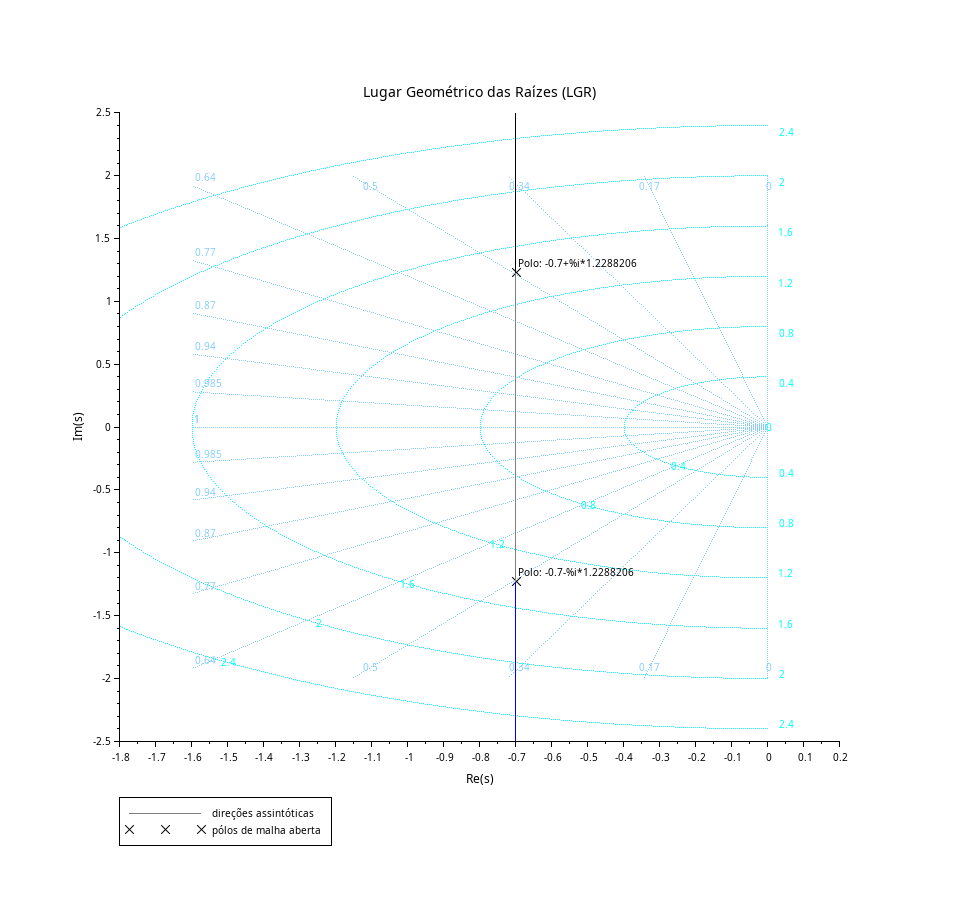
\includegraphics[width=0.8\textwidth]{atividades/7-atividade/assets/lgr.png}
    \caption{Lugar Geométrico das Raízes do sistema massa-mola-amortecedor.}
    \label{fig:LGR}
\end{figure}

Esta análise do Lugar Geométrico das Raízes (LGR) sugere uma tendência do sistema de manter a estabilidade diante de variações nos parâmetros, embora essa interpretação dependa de suposições sobre as condições de contorno e a natureza das mudanças paramétricas. As propriedades observadas nos pólos e nas assíntotas, particularmente sua simetria, fornecem indícios importantes para o design de sistemas de controle. No entanto, é essencial considerar que a visualização por meio do LGR oferece uma perspectiva limitada, que precisa ser complementada com outras análises dinâmicas para validar completamente a estabilidade e a eficácia do controle em cenários variados.

\begin{itemize}
    \item \textbf{Pólos e Simetria:}
          Os pólos do sistema, identificados claramente no LGR como \( s = -0.35 \pm j1.228\) (como mostrado na imagem com precisão real e imaginária), indicam uma resposta subamortecida do sistema devido ao posicionamento no semiplano esquerdo. A configuração destes pólos no semiplano esquerdo sugere uma estabilidade inerente sem oscilações não amortecidas.
          
    \item \textbf{Estabilidade e Assíntotas:}
          O sistema exibe duas assíntotas calculadas a partir da posição dos polos, indicando um movimento vertical dos pólos no plano complexo com o aumento do ganho do controlador. Estas assíntotas estão orientadas a \(90^\circ\) e \(-90^\circ\), garantindo que qualquer aumento nos parâmetros de controle mantenha a estabilidade desde que os pólos não cruzem o eixo imaginário.

    \item \textbf{Considerações sobre a Estabilidade:}
          A análise do LGR confirma a estabilidade do sistema com os pólos localizados estritamente no semiplano esquerdo. Entretanto, para garantir a validade dessa estabilidade sob diversas condições operacionais, sugere-se realizar análises adicionais como a de Nyquist ou Bode para avaliar a resposta do sistema frente a uma gama mais ampla de variações paramétricas.
\end{itemize}



 % Completo e Validado
\section{Atividade 8}

\subsection{Análise do Diagrama de Bode}

A Figura \ref{fig:Bode} apresenta o diagrama de Bode do sistema massa-mola-amortecedor com os parâmetros \(M = 10\), \(C = 7\), e \(K = 5\). O diagrama de Bode fornece informações valiosas sobre a resposta em frequência do sistema e é composto por dois gráficos: magnitude e fase.

\begin{itemize}
    \item \textbf{Gráfico de Magnitude:}
          O gráfico de magnitude, expresso em decibéis (dB), mostra que a magnitude aumenta inicialmente, atinge um pico em uma determinada frequência e depois decresce. Este comportamento indica a presença de ressonância no sistema, onde a resposta do sistema é maximizada em uma certa frequência.

    \item \textbf{Gráfico de Fase:}
          O gráfico de fase, expresso em graus, apresenta uma variação típica que começa em 0 graus, decresce através de -90 graus e se aproxima de -180 graus em frequências mais altas. A variação da fase indica a diferença de fase entre a entrada e a saída do sistema em diferentes frequências.

    \item \textbf{Margens de Ganho e Fase:}
          \begin{itemize}
              \item \textbf{Margem de Ganho:} A margem de ganho é a quantidade de ganho adicional que o sistema pode tolerar antes de se tornar instável. No gráfico, se a magnitude na frequência onde a fase é -180 graus estiver abaixo de 0 dB, a margem de ganho é positiva e o sistema é estável.
              \item \textbf{Margem de Fase:} A margem de fase é a quantidade de fase adicional que o sistema pode tolerar antes de se tornar instável. No gráfico, se a fase na frequência onde a magnitude é 0 dB estiver acima de -180 graus, a margem de fase é positiva e o sistema é estável.
          \end{itemize}
\end{itemize}

\begin{figure}[h]
    \centering
    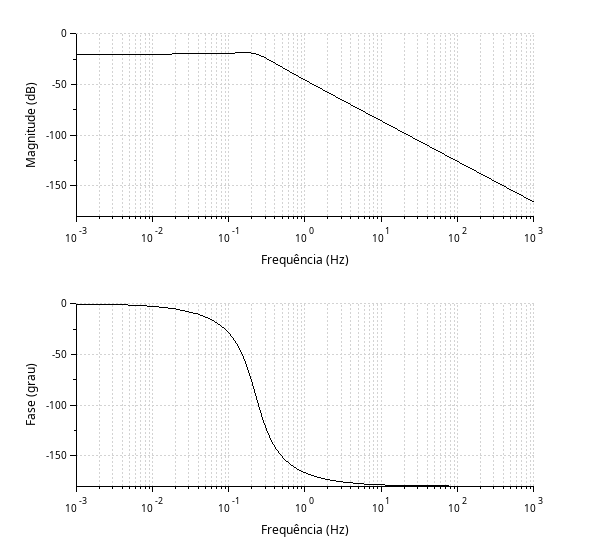
\includegraphics[width=0.8\textwidth]{atividades/8-atividade/assets/bode.png}
    \caption{Diagrama de Bode do sistema massa-mola-amortecedor.}
    \label{fig:Bode}
\end{figure}

A análise do diagrama de Bode sugere que o sistema é estável para as frequências observadas. As margens de ganho e fase indicam que o sistema pode tolerar variações razoáveis no ganho e na fase sem perder a estabilidade. No entanto, é importante considerar que esta análise deve ser complementada com outras técnicas de análise de estabilidade para garantir uma avaliação completa.
 % Completo e Validado
\section{Atividade 9}

\subsection{Análise do Diagrama de Nyquist}

O diagrama de Nyquist é uma ferramenta essencial para visualizar a resposta em frequência da função de transferência de malha aberta e para avaliar a estabilidade do sistema em malha fechada. A seguir, analisamos a estabilidade geral do sistema e as margens de ganho e fase, utilizando o diagrama de Nyquist para o sistema massa-mola-amortecedor com parâmetros \(M = 10\), \(C = 7\), e \(K = 5\).

\subsubsection{Diagrama de Nyquist e Estabilidade do Sistema}

\begin{figure}[H]
    \centering
    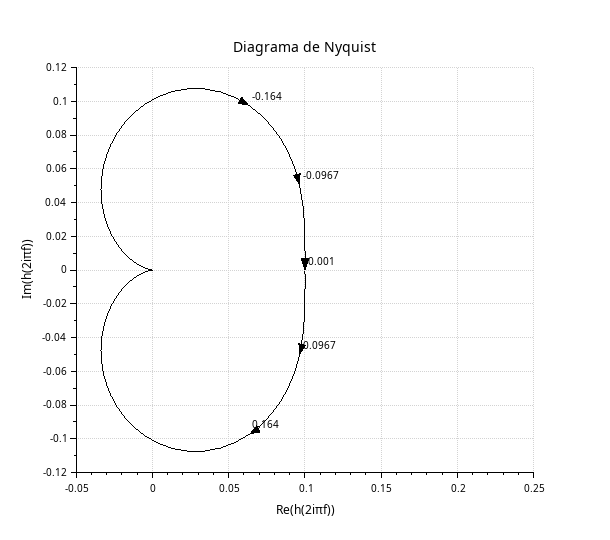
\includegraphics[width=0.8\textwidth]{atividades/9-atividade/assets/nyquist.png}
    \caption{Diagrama de Nyquist do sistema massa-mola-amortecedor.}
    \label{fig:Nyquist1}
\end{figure}

Na Figura \ref{fig:Nyquist1}, observamos que a trajetória da curva em relação ao ponto crítico \(-1 + 0j\) não circunda este ponto, indicando que o sistema é estável em malha fechada. Este comportamento sugere que o sistema não atingirá instabilidade sob condições normais de operação.

\subsubsection{Interpretação Geométrica e Estabilidade}

O diagrama mapeia a resposta complexa da função de transferência ao longo de uma gama de frequências no plano complexo. Este mapeamento é crucial para aplicar o critério de Nyquist:
\begin{itemize}
    \item A curva não encircla o ponto \(-1\), confirmando a estabilidade em malha fechada segundo o Princípio do Argumento.
    \item A proximidade da curva ao ponto crítico ajuda a determinar a margem de estabilidade antes que ganhos adicionais possam induzir instabilidade.
\end{itemize}

\subsubsection{Análise de Polos e Zeros e Margens de Ganho e Fase}

\begin{figure}[H]
    \centering
    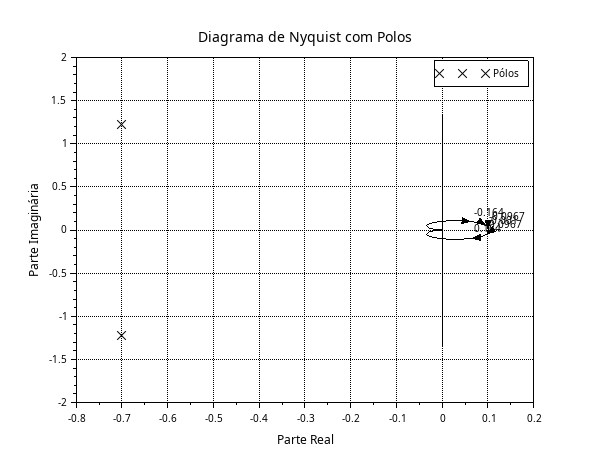
\includegraphics[width=0.8\textwidth]{atividades/9-atividade/assets/nyquist-com-polos.png}
    \caption{Diagrama de Nyquist com visualização de polos do sistema massa-mola-amortecedor.}
    \label{fig:NyquistPolos}
\end{figure}

A Figura \ref{fig:NyquistPolos} mostra a localização dos polos, marcados com 'X', no diagrama de Nyquist, oferecendo insights adicionais sobre como os polos e zeros influenciam a estabilidade e resposta do sistema:
\begin{itemize}
    \item Os polos no semiplano esquerdo confirmam a estabilidade, enquanto sua proximidade ao eixo imaginário pode indicar sensibilidade a perturbações.
    \item As margens de ganho e fase podem ser visualmente estimadas pela distância e ângulo da curva em relação ao ponto \(-1 + 0j\), sugerindo que o sistema possui uma margem de segurança robusta para tolerar variações nos parâmetros de controle.
\end{itemize}

\subsubsection{Análise Quantitativa das Margens de Ganho e Fase}
A margem de ganho é crucial para determinar quão perto o sistema está de atingir a instabilidade sob aumento de ganho. No Diagrama de Nyquist, a distância mínima do ponto \(-1 + 0j\) até a curva pode ser visualmente estimada e, em casos práticos, calculada utilizando software específico. Por exemplo, uma distância de 0.5 unidades no diagrama pode indicar que o ganho pode ser aumentado em até 50\% antes de o sistema se tornar instável.

Da mesma forma, a margem de fase é determinada calculando o ângulo que falta para que a curva passe exatamente pelo ponto \(-1 + 0j\). Um ângulo de margem de fase de 30° sugere que uma mudança de fase de até 30° ainda manteria o sistema estável. A análise detalhada dessas margens ajuda a prever e evitar cenários de instabilidade em aplicações práticas.

\subsubsection{Conclusão}
A análise combinada dos diagramas de Nyquist reforça a percepção de estabilidade do sistema, indicando amplas margens de ganho e fase. No entanto, é recomendável complementar esta análise com outras técnicas de análise de estabilidade, como diagramas de Bode ou análise de lugar das raízes, para uma avaliação mais abrangente da robustez do sistema. Essas técnicas adicionais ajudarão a confirmar as descobertas e a proporcionar uma compreensão mais completa das dinâmicas do sistema sob diferentes condições de operação.
  % Completo e Validado
\section{Atividade 10}

\subsection{Identificação de Sistemas}

Nesta atividade, abordamos a identificação do sistema representado pela função de transferência especificada na Atividade 3. Utilizando a resposta ao degrau unitário, aplicamos os métodos de Harriot e Smith para identificar os parâmetros de um sistema de segunda ordem. Os resultados obtidos por cada método serão comparados para determinar qual fornece uma identificação mais precisa das características do sistema.

Para otimizar a análise e assegurar que os resultados sejam imediatamente interpretáveis, adotamos um degrau de entrada com amplitude 5. Este ajuste estratégico evita a complexidade associada à normalização posterior dos dados, garantindo que a amplitude da resposta permaneça normalizada em 1 ao longo do tempo.

A Figura \ref{fig:diagrama-sistema} ilustra a resposta ao degrau unitário do sistema massa-mola-amortecedor, especificado pelos parâmetros \(M = 10\), \(C = 7\), e \(K = 5\). Essa resposta é crucial para a identificação dos parâmetros do sistema utilizando os métodos de Harriot e Smith, permitindo uma análise detalhada da dinâmica do sistema em resposta a perturbações externas.

\begin{figure}[h]
    \centering
    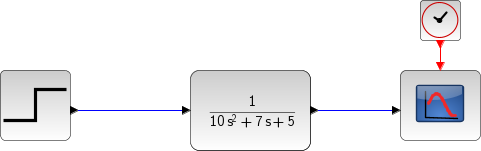
\includegraphics[width=0.8\textwidth]{atividades/10-atividade/assets/diagrama-sistema.png}
    \caption{Resposta ao degrau unitário do sistema massa-mola-amortecedor.}
    \label{fig:diagrama-sistema}
\end{figure}

Utilizando a ferramenta DataTip, marcamos pontos significativos na curva de resposta correspondentes a 20\%, 60\%, 73\% e 100\% do valor final. Estes pontos são essenciais para a aplicação dos métodos de identificação, pois fornecem dados precisos sobre a resposta do sistema em diferentes fases do seu comportamento transitório.

A Figura \ref{fig:sistema-identificado-forcado-normalizado} apresenta a resposta ao degrau unitário com os parâmetros identificados segundo os métodos de Harriot e Smith, destacando a utilidade dessas metodologias na análise de sistemas dinâmicos.

\begin{figure}[h]
    \centering
    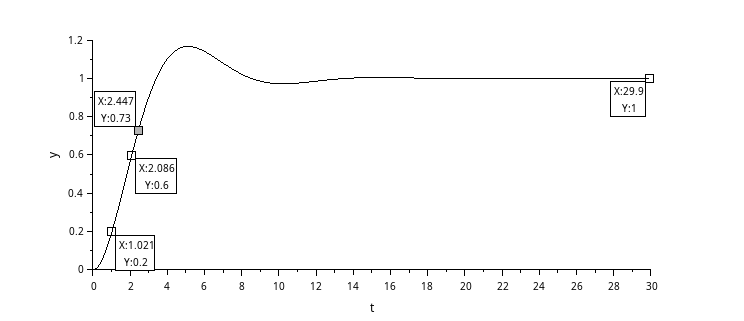
\includegraphics[width=0.8\textwidth]{atividades/10-atividade/assets/sistema-identificado-forcado-normalizado.png}
    \caption{Identificação dos parâmetros do sistema com a resposta ao degrau unitário, ilustrando a eficácia dos métodos de Harriot e Smith.}
    \label{fig:sistema-identificado-forcado-normalizado}
\end{figure}

\subsection{Aplicação do Método de Harriot}

O Método de Harriot é tradicionalmente empregado para identificar os parâmetros de sistemas de primeira ordem, focando na constante de tempo (\(\tau\)) e no ganho do sistema (\(K\)). Este método analisa como o sistema responde a um degrau unitário para extrair esses parâmetros. Para esta análise específica, optou-se por aplicar um degrau de amplitude 5, facilitando a interpretação dos resultados ao evitar a normalização posterior. Duas abordagens principais foram consideradas:

\begin{enumerate}
    \item \textbf{Utilização direta do degrau de amplitude 5:} Esta abordagem aproveita a amplitude do degrau para manter os dados experimentais alinhados com o sistema real, sem a necessidade de ajustes adicionais para a normalização.
    \item \textbf{Normalização para um degrau unitário:} Caso um degrau unitário tivesse sido aplicado, seria necessário normalizar os valores de resposta dividindo-os pelo valor final esperado (\(5K\)), adaptando a análise às fórmulas padrão do Método de Harriot.
\end{enumerate}

\subsubsection{Cálculo da Constante de Tempo}

A constante de tempo crítica para a aplicação do Método de Harriot foi determinada como segue:
\[
    \tau = 0.5 \cdot \frac{t_{73}}{1.3} = 0.5 \cdot \frac{2.449}{1.3} \approx 0.9419 \text{ segundos}
\]

Os pontos de resposta ao degrau usados para esta análise incluem:
\begin{itemize}
    \item \(X = 1.022\), \(Y = 0.2\) (20\% do valor final).
    \item \(X = 2.094\), \(Y = 0.6\) (60\% do valor final).
    \item \(X = 2.449\), \(Y = 0.73\) (73\% do valor final).
    \item \(X = 29.9\), \(Y = 1\) (100\% do valor final).
\end{itemize}

\subsubsection{Limitação do Método de Harriot}

Uma limitação significativa do Método de Harriot é sua aplicabilidade principalmente a sistemas sobreamortecidos. No entanto, o sistema em análise é subamortecido. Além disso, para uma eficaz aplicação do método, a razão \(Y/KM\) deve ser maior que 0.26 após a normalização para uma resposta ao degrau unitário. No presente caso, o valor de \(Y/KM\) calculado foi 0.175, indicando que o Método de Harriot não é adequado para esta configuração específica. Portanto, são recomendadas abordagens alternativas de identificação ou ajustes na configuração experimental.

\begin{figure}[h]
    \centering
    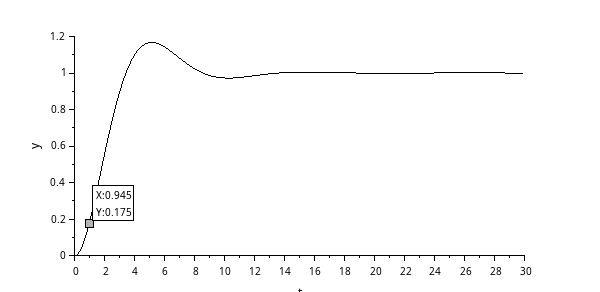
\includegraphics[width=0.8\textwidth]{atividades/10-atividade/assets/sistema-t73-identificado-nromalizacao-forcada.png}
    \caption{Identificação do sistema massa-mola-amortecedor utilizando o Método de Harriot.}
    \label{fig:sistema-t73-identificado-nromalizacao-forcada}
\end{figure}

A Figura \ref{fig:sistema-t73-identificado-nromalizacao-forcada} ilustra a tentativa de aplicação do Método de Harriot, destacando que a inadequação dos parâmetros extraídos confirma as limitações do método para este caso específico. Esta análise sugere a necessidade de explorar métodos alternativos que sejam mais compatíveis com as características dinâmicas do sistema subamortecido em estudo.

\subsection{Aplicação do Método de Smith}

O Método de Smith é uma técnica avançada que utiliza a resposta ao degrau unitário para estimar a frequência natural (\(\omega_n\)) e o fator de amortecimento (\(\zeta\)) de um sistema. Este método é particularmente útil para a análise de sistemas de segunda ordem, proporcionando uma visão clara das características dinâmicas do sistema a partir de sua resposta temporal.

\subsubsection{Análise de Razão Temporal}

Inicialmente, calculamos a razão entre os tempos que correspondem a 20\% e 60\% da resposta final do degrau. A razão é calculada usando a fórmula:
\[
    \frac{t_{20}}{t_{60}} = \frac{1.022}{2.086} \approx 0.461706
\]
Esta métrica é crucial porque define a trajetória no gráfico de Smith para deduzir os valores de \(\zeta\) e \(\tau\).

\subsubsection{Interpretação Gráfica}

Utilizando a razão calculada, consultamos o gráfico do Método de Smith, conforme ilustrado na Figura \ref{fig:analise-smith}. Este gráfico correlaciona \(\frac{t_{20}}{\tau}\) e \(\frac{t_{60}}{\tau}\) com os valores de \(\zeta\) e \(\tau\), facilitando a interpretação direta das características do amortecimento e da constante de tempo do sistema. É importante notar que o gráfico apresenta dois eixos Y: o da esquerda mostra \(\frac{t_{60}}{\tau}\) enquanto o da direita exibe valores para \(\zeta\).

\begin{figure}[h]
    \centering
    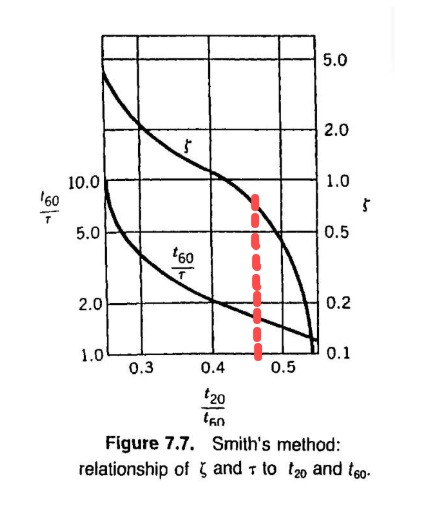
\includegraphics[width=0.8\textwidth]{atividades/10-atividade/assets/analise-smith.png}
    \caption{Gráfico utilizado no Método de Smith: relação entre \(\zeta\) e \(\tau\) com \(\frac{t_{20}}{\tau}\) e \(\frac{t_{60}}{\tau}\).}
    \label{fig:analise-smith}
\end{figure}

Através deste gráfico, identificamos que a razão \(\frac{t_{60}}{\tau}\) para nossa razão específica \(\frac{t_{20}}{t_{60}}\) é aproximadamente 1.8. Com esta informação, podemos calcular \(\tau\) usando o tempo conhecido \(t_{60}\):
\[
    \tau = \frac{t_{60}}{1.8} = \frac{2.086}{1.8} \approx 1.159 \text{ segundos}
\]

\subsubsection{Cálculo de Parâmetros do Sistema}

Com o \(\tau\) calculado, podemos inferir \(\zeta\) diretamente do gráfico e aplicar esses valores na função de transferência do sistema:
\[
    G(s) = \frac{Kp}{\tau^2 s^2 + 2 \zeta \tau s + 1} = \frac{Kp}{(1.159)^2 s^2 + 2 \zeta (1.159) s + 1}
\]

\subsubsection{Limitações e Recomendações}

A análise conduzida através do Método de Smith, apesar de instrutiva, enfrenta limitações significativas devido ao uso de uma representação gráfica baseada em imagem. A precisão dos valores obtidos pode ser comprometida por ruídos visuais e erros de interpretação. Para resultados mais confiáveis, é recomendável o uso de gráficos dinâmicos gerados diretamente de dados experimentais, minimizando a interpretação visual e os erros associados.


\subsection{Comparação dos Métodos e Conclusão}

A avaliação dos métodos de Harriot e Smith revelou nuances importantes no processo de identificação de sistemas. Cada método demonstra forças e limitações que são cruciais ao considerar a adequação ao tipo específico de sistema analisado.

\subsubsection{Método de Harriot}
O Método de Harriot, tradicionalmente adequado para sistemas sobreamortecidos, encontrou dificuldades significativas de aplicação ao sistema subamortecido em estudo. Além disso, o indicador chave para a aplicação do método, a razão \(Y/KM\), mostrou-se insuficiente (\(0.175\)), ficando bem abaixo do limite necessário (\(0.26\)) para uma identificação eficaz. Isso sugere que o Método de Harriot pode não ser a escolha ideal para sistemas que não se enquadram claramente em configurações sobreamortecidas, ou quando a resposta ao degrau não alcança um platô claro e definido.

\subsubsection{Método de Smith}
O Método de Smith, por outro lado, é mais flexível para sistemas subamortecidos, oferecendo insights sobre a frequência natural e o fator de amortecimento. No entanto, a análise dependente de uma representação gráfica visual introduz um nível de incerteza, especialmente quando os dados são interpretados a partir de uma imagem estática, que pode incorporar ruídos e distorções visuais. Tais fatores podem afetar a precisão dos parâmetros inferidos, limitando a confiabilidade das conclusões.

\subsubsection{Considerações Finais e Recomendações}
Em face das análises realizadas e das limitações observadas em ambos os métodos, conclui-se que a identificação dos parâmetros do sistema não foi alcançada de maneira confiável e satisfatória. As incertezas e as inadequações metodológicas levam à recomendação de que outras abordagens sejam consideradas para uma identificação mais precisa. Métodos alternativos, possivelmente combinando aspectos quantitativos e qualitativos, ou mesmo ajustes na configuração experimental, podem ser necessários para garantir resultados mais robustos e verificáveis.

Concluímos que, diante das circunstâncias e resultados, é mais prudente não afirmar com certeza a identificação dos parâmetros do sistema. Em vez disso, recomenda-se explorar outras técnicas e metodologias, talvez integrando dados adicionais ou utilizando software de simulação avançada, para obter uma compreensão mais profunda e precisa das dinâmicas do sistema.

Este caso destaca a importância de escolher o método apropriado para o tipo de sistema e resposta observada e sugere que a cautela seja um componente crucial ao interpretar e aplicar técnicas de identificação em engenharia de controle.
 % Completo e Validado

% ===============================================================
% Conclusão geral ===============================================
\section{Conclusão Geral}

Este projeto abordou uma série de atividades fundamentais para a modelagem e controle de sistemas dinâmicos, especificamente um sistema massa-mola-amortecedor. Cada atividade teve um papel crucial na compreensão e aplicação dos princípios de controle e simulação.

Inicialmente, desenvolvemos um script no Scilab para modelar o sistema massa-mola-amortecedor com força de entrada nula, simulando o sistema para diferentes condições iniciais. Esta atividade foi essencial para entender como o sistema responde naturalmente a diferentes estados iniciais sem a influência de forças externas. Observamos como a velocidade inicial e a posição inicial afetam o comportamento transiente do sistema e a importância do amortecimento na estabilização do sistema.

Em seguida, utilizamos o Xcos para criar um diagrama de blocos que simula o sistema com uma força de entrada constante. Esta atividade destacou a importância das ferramentas de simulação visual e como elas podem facilitar a compreensão do comportamento do sistema sob diferentes condições iniciais e entradas de força. Identificamos parâmetros transientes cruciais, como tempo de subida, tempo de pico, tempo de estabelecimento e estado estacionário.

A construção da função de transferência do sistema e a determinação dos polos e parâmetros típicos de um sistema de segunda ordem (\(k_p\), \(\omega_n\) e \(\zeta\)) proporcionaram uma base sólida para a análise de estabilidade e resposta do sistema. Esta atividade foi vital para compreender a relação entre os parâmetros físicos do sistema e sua resposta dinâmica, bem como para preparar o terreno para as atividades subsequentes de controle.

Modelamos um sistema de controle com um controlador proporcional e analisamos sua estabilidade utilizando o critério de Routh-Hurwitz. Esta atividade sublinhou a importância de uma análise rigorosa de estabilidade para garantir que o sistema responda de maneira controlada e previsível. A construção da matriz de Routh-Hurwitz e a determinação dos limites de estabilidade para diferentes valores de \(K\) forneceram insights valiosos sobre a robustez do sistema.

Simulamos o sistema de controle proporcional utilizando o Xcos e analisamos a resposta do sistema a um sinal de degrau. Esta atividade demonstrou como ajustes no ganho do controlador afetam a resposta do sistema, mostrando a necessidade de um equilíbrio entre resposta rápida e estabilidade. A análise comparativa entre diferentes configurações de ganho destacou os trade-offs envolvidos no ajuste de controladores.

A introdução de um controlador PID, ajustado através do método de Ziegler-Nichols, e a comparação com o controlador proporcional enfatizaram as vantagens do controle PID em termos de precisão e estabilidade. Esta atividade foi crucial para demonstrar como a combinação de ações proporcional, integral e derivativa pode melhorar significativamente a performance do sistema, especialmente em condições operacionais variadas.

Desenhamos o lugar geométrico das raízes para a planta utilizando o Scilab, o que nos permitiu visualizar como as raízes do sistema se deslocam no plano complexo à medida que o ganho do controlador varia. Esta atividade forneceu uma compreensão visual poderosa da estabilidade e das características de resposta do sistema.

A análise dos diagramas de Bode forneceu informações essenciais sobre a frequência de resposta do sistema, incluindo margens de ganho e fase. Esta atividade destacou a importância da análise de frequência para o design de controladores que garantam estabilidade e performance robusta em uma ampla faixa de frequências.

O diagrama de Nyquist ofereceu uma abordagem gráfica para avaliar a estabilidade do sistema em malha fechada. Esta atividade complementou a análise de Bode e Routh-Hurwitz, proporcionando uma visão abrangente sobre a robustez do sistema de controle.

A identificação de sistemas através da resposta ao degrau e dos métodos de Harriot e Smith permitiu validar o modelo matemático do sistema. Esta atividade destacou a importância de técnicas de identificação para garantir que os modelos utilizados reflitam com precisão o comportamento real do sistema.

As atividades desenvolvidas ao longo deste projeto foram fundamentais para uma compreensão aprofundada dos princípios de modelagem e controle de sistemas dinâmicos. Cada atividade contribuiu para o desenvolvimento de habilidades práticas em simulação, análise de estabilidade e ajuste de controladores, fornecendo uma base sólida para aplicações práticas em engenharia. Através dessas atividades, foi possível observar a importância da escolha adequada de parâmetros e técnicas de controle para garantir a estabilidade e a performance desejada em sistemas reais.


% ===============================================================
% Referencias ===================================================
\begin{titlepage}
    \setstretch{1.5} % Espaçamento entre linhas, certifique-se de que o pacote setspace está incluído em document.tex

    \section{Referências}

    \vspace{0.5cm} % Espaço vertical

    \noindent OGATA, Katsuhiko. \textbf{Modern Control Engineering}. 5. ed. Upper Saddle River, NJ: Prentice Hall, 2010.

    \noindent NISE, Norman S. \textbf{Control Systems Engineering}. 7. ed. Hoboken, NJ: John Wiley \& Sons, 2015.

    \noindent ZIEGLER, John G.; NICHOLS, Nathaniel B. Optimum Settings for Automatic Controllers. \textbf{Transactions of the ASME}, v. 64, p. 759-768, 1942.

    \noindent SCILAB ENTERPRISES. \textbf{Scilab: Free and Open Source Software for Numerical Computation}. Versão 6.1.0, 2020. Disponível em: <https://www.scilab.org>. Acesso em: 14 jun. 2024.

    \noindent SCILAB ENTERPRISES. \textbf{Xcos: Hybrid dynamic systems modeler and simulator}. Versão 1.0, 2020. Disponível em: <https://www.scilab.org/software/xcos>. Acesso em: 14 jun. 2024.

\end{titlepage}

% ===============================================================
% Anexo ou Apendices ============================================
\begin{titlepage}
    \setstretch{1.5} % Espaçamento entre linhas, certifique-se de que o pacote setspace está incluído em document.tex

    \section{Apendice}

    % \subsection{Atividade 1 - Código}
    % \lstinputlisting[language=Matlab, caption={Código Scilab para Simulação do Sistema Massa-Mola-Amortecedor}]{atividades/1-atividade/scilab/final-code.sce}
\end{titlepage}

% ===============================================================
% End Document ==================================================
\end{document}

